% kappa.tex
% STOLAR: Form Follows Fitness
% Kappa-tekst for artikkelbasert avhandling
% Spraak: Nynorsk

\documentclass[10pt, a4paper, twocolumn]{article}

\usepackage[utf8]{inputenc}
\usepackage[T1]{fontenc}
\usepackage[nynorsk]{babel}
\usepackage{mathpazo}
\usepackage{amsmath, amssymb}
\usepackage{booktabs}
\usepackage{graphicx}
\usepackage{xcolor}
\usepackage{hyperref}
\usepackage[round]{natbib}
\usepackage{setspace}
\usepackage{geometry}
\usepackage{csquotes}
\usepackage{float}
\usepackage{enumitem}

\geometry{margin=1.5cm, top=1.8cm, bottom=1.8cm, columnsep=0.6cm}
\setstretch{1.05}
\usepackage{pdfpages}
\graphicspath{{fig/}}

\title{%
  \vspace{-2cm}
  {\large Arkitektur- og designhøgskolen i Oslo}\\
  {\large Institutt for design}\\[2cm]
  {\Huge\textbf{STOLAR}}\\[0.5em]
  {\LARGE Form Follows Fitness}\\[0.5em]
  {\large Kvantitativ analyse av europeisk stoldesign, 1280--2024}\\[3cm]
  {\normalsize Iver Raknes Finne}\\[0.5em]
  {\small Masteroppgåve i design}\\
  {\small Våren 2026}\\[1em]
  {\small Rettleiar: [rettleiarnamn]}
}
\author{}
\date{}

\begin{document}
\maketitle
\thispagestyle{empty}
\newpage

% ================================================================
\begin{abstract}
\noindent Denne avhandlinga undersøkjer empirisk om Louis Sullivan sitt aksiom ``form ever follows function'' held mot eit reelt datasett. Gjennom kvantitativ analyse av 2\,284 stolar frå Nasjonalmuseet for kunst, arkitektur og design og Victoria \& Albert Museum, registrerte mellom 1280 og 2024, byggjer avhandlinga ein kumulativ beviskjede over fire artiklar.

\emph{Artikkel~I} avdekkjer at materialar ikkje er nøytrale medium, men komprimerte geopolitiske historier: Shannon-entropien stig monotont frå $H' = 1{,}0$ til 5,07 bits over 700 år. \emph{Artikkel~II} viser at dimensjonar driftar under geografisk og teknologisk påverknad, med systematisk negative Modulor-avvik ($-18$ til $-40$ cm). \emph{Artikkel~III} demonstrerer at dimensjonar og materialkombinasjonar predikerer stilperiode med $F1 = 0{,}823$ og nasjonalitet med $F1 = 0{,}721$, medan stilmerket åleine er den svakaste prediktoren for faktisk geometri. \emph{Artikkel~IV} samlar bevisa og formulerer \textbf{Form Follows Fitness} (FFF) som eit koherent alternativ: form er ikkje dedusert frå funksjon, men selektert av eit fleirdimensjonalt tilpassingslandskap der materiale, teknologi, økonomi, geografi og kultur alle utøver seleksjonstrykk.

Kappa-teksten syntetiserer beviskjeda, demonstrerer at FFF er eit paradigmeskifte i Kuhn sin tyding, og viser at rammeverket generaliserer frå stolar til alle estetiske fag. Ein proposisjonell traktat formaliserer dei sju kardinale prinsippa i FFF.

\medskip
\noindent\textbf{Nøkkelord:} Form Follows Fitness, fitnesslandskap, stoldesign, kvantitativ designhistorie, materialaffordanse, seleksjonstrykk, Shannon-entropi
\end{abstract}

\newpage
\tableofcontents
\newpage


% ================================================================
\section{Innleiing: ein revolusjon i fire akter}

\begin{quote}
``It is the pervading law of all things organic and inorganic [\ldots] that \emph{form ever follows function}. This is the law.'' \citep{sullivan1896}
\end{quote}

\subsection{To stolar, 550 år}

I 1280, i eit uoppvarma langhus i Bø i Telemark, sat ein mann på ein stol skoren av lokal bjørk med enkel tapping og grove proporsjonar. Stolen er i dag katalogisert som OK-10700 i Nasjonalmuseet si samling. Han måler 98 cm i høgde, 42 cm i breidde, og veg anslagsvis 14 kg. Materialpaletten er eitt einaste treslag; verktøyspråket er øks, kniv og telje. Funksjonen er eksakt den same som for alle andre stolar i dette datasettet: å bere ein sitjande kropp.

Femhundreogfemti år seinare, i 1830, vart ein annan stol produsert. OK-10330A er ein empirestol i mahogni, silketrekk og bladgull, truleg importert til Noreg frå eit dansk eller nordtysk verkstad. Han måler 84 cm i høgde, 48 cm i breidde, og veg anslagsvis 8 kg. Materiala hans fortener ein heil geopolitisk roman: mahognien kjem frå Honduras via Liverpool, silken frå Lyon, bladgullet frå eit hammarslått gullverk. Funksjonen er den same.

Desse to stolane deler éin invariant eigenskap og divergerer i nær sagt alt anna. Funksjonen er identisk; forma er radikalt ulik. Dersom Sullivan sitt aksiom var sant, skulle to objekt med same funksjon konvergere mot same form. Dei gjer det ikkje. Ikkje mellom OK-10700 og OK-10330A, ikkje mellom nokon av dei 2\,284 stolane i dette datasettet. Spørsmålet er kvifor.

\subsection{Bakgrunn og motivasjon}

I over eit hundreår har Louis Sullivan sitt aksiom fungert som grunnlova i formgjevingsfaga. \citet{lecorbusier1923} bygde ein arkitektonisk doktrine på premissen. \citet{alexander1964} foreslo systematisk formderivering frå funksjonskrav. \citet{giedion1948} dokumenterte mekaniseringa som den naturlege utfaldinga av funksjonell logikk. \citet{forty1986} kritiserte designideologiar, men tilbaud ikkje eit kvantitativt alternativ. \citet{raizman2010} skreiv standardhistoria om moderne design utan å teste premissane empirisk. Ingen stilte spørsmålet med tal.

Denne avhandlinga stiller det. Metoden er enkel: samle alle stolar med same funksjon, måle dei, og sjå om formvariasjonen er liten nok til å støtte aksiomet. Ho er ikkje det. Variasjonen er massiv, systematisk og korrelert med variablar som ikkje har noko med funksjon å gjere: materiale, geografi, tid, teknologi, handelsvegar og kulturelle konvensjonar.

\subsection{Datamaterialet}

STOLAR-databasen inneheld 2\,284 stolar frå to europeiske museumssamlingar: Nasjonalmuseet for kunst, arkitektur og design (NMK) i Oslo ($n = 671$), og Victoria \& Albert Museum (V\&A) i London ($n = 1\,613$). Tidsrommet strekkjer seg frå 1280 til 2024. Alle objekta deler same invariante funksjon: å bere ein sitjande kropp.

Kvar stol er dokumentert med dimensjonsvariablar (høgde, breidde, djupn, setehøgde), materiallister, teknikkar, stilmerke (22,9\,\% dekning), nasjonalitet (70,2\,\% dekning) og produksjonsår. Datasettet registrerer 76 unike materialar, 38 teknikkar, 24 stilperiodar og 12 produksjonsland. Materialpaletten strekkjer seg frå lokal bjørk og furu i mellomalderen til karbonfiber og resirkulert plast i samtida. Teknikkane spenner frå handskjering og tapping til CNC-fresing og sprøytestøyping. Dei 12 landa dekkjer kjernelanda i den europeiske møbeltradisjon, frå Storbritannia og Frankrike til Noreg, Danmark og Sverige, med innslag frå Italia, Tyskland, Austerrike og USA.

\subsection{Forskingsspørsmål}

Avhandlinga stiller fem spørsmål:
\begin{enumerate}
  \item Er formvariasjonen stor nok til å falsifisere funksjonsdeterminismen?
  \item Kva seleksjonstrykk forklarer mest formvariasjon?
  \item Er stilperiode ei årsak til form, eller eit emergent restprodukt?
  \item Korleis endrar tilpassingslandskapet seg over tid?
  \item Kan ein formulere eit empirisk testbart alternativ til funksjonalismen?
\end{enumerate}

Dei korte svara, som artiklane utdjupar fullt ut, er: (1) Ja, formvariasjonen er massiv: gjennomsnittleg høgde varierer med ein faktor 1,6, estimert vekt med ein faktor 7, og materialpaletten med 76 unike kategoriar. (2) Materiale og proporsjonar ber til saman meir enn fire gonger så mykje informasjon om stilperiode som funksjon (MI = 2,072 bits mot 0,000 bits). (3) Stilperiode er eit emergent restprodukt: Random Forest-modellen predikerer stilperiode med $F1 = 0{,}823$ frå dimensjonar og materialar, men stilmerket åleine er den svakaste prediktoren for faktisk geometri. (4) Landskapet endrar seg mest ved materialregimeskifte: frå lokalt tre ($H' < 2$ bits) via kolonialt handelstre ($H' \approx 3{,}5$ bits) til industrielle og syntetiske materialar ($H' = 5{,}07$ bits). (5) Ja: Form Follows Fitness (FFF) subsumerer funksjonalismen som eit degenerert spesialtilfelle, gyldig berre når alle seleksjonstrykk utanom funksjon er eksakt lik null.

\subsection{Avhandlingsstruktur}

Avhandlinga er artikkelbasert. Fire artiklar utgjer beviskjeda; denne kappa-teksten syntetiserer dei til ei samanhengande forteljing og presenterer det overordna teoretiske rammeverket, Form Follows Fitness. Kapittel~2 etablerer det teoretiske fundamentet gjennom fem tverrvitskaplege pilarar. Kapittel~3 beskriv metoden, datamaterialet og dei statistiske verktøya. Kapittel~4 samanfattar kvar artikkel med vekt på dei kvantitative funna. Kapittel~5 presenterer den overordna syntesen og viser korleis beviskjeda oppfyller Kuhn sine kriterium for paradigmeskifte. Kapittel~6 inneheld ein proposisjonell traktat som formaliserer FFF i sju hovudproposisjonar med underproposisjonar. Kapittel~7 konkluderer med implikasjonar for praksis, utdanning og vidare forsking.


% ================================================================
\section{Teoretisk rammeverk: fem pilarar}

Rammeverket Form Follows Fitness kviler på fem tverrvitskaplege pilarar. Ingen av dei er nye i seg sjølve; det nye er syntesen. Kvar pilar er henta frå eit anna fagfelt, frå evolusjonsbiologi og kognitiv vitskap til økologi og paleontologi, og saman utgjer dei eit rammeverk som er rikare og meir empirisk forankra enn noko einskild tradisjon kan tilby åleine. I det følgjande presenterer eg kvar pilar, dei teoretiske røtene, og korleis pilaren manifesterer seg i STOLAR-dataa.

\subsection{Fitnesslandskapet}

\citet{wright1932} introduserte omgrepet \textbf{fitnesslandskap} som ein topografisk modell av evolusjonær tilpassing. Wright førestilte seg eit fleirdi\-men\-sjonalt terreng der kvar posisjon svarar til ein genotype, og høgda over havet svarar til fitness, altså overlevings- og reproduksjonssukses. \citet{kauffman1993} utvida modellen til såkalla $NK$-landskap, der $N$ er talet på komponentar og $K$ er talet på epistatiske interaksjonar mellom dei. Kauffman viste at når $K$ aukar, vert landskapet meir ruglete: talet på lokale toppunkt veks eksponentielt, og global optimalisering vert tilnærma umogleg.

I FFF er forma ein posisjon i eit $n$-dimensjonalt landskap der kvar akse representerer eit seleksjonstrykk: materiale, teknologi, økonomi, geografi, kulturell konvensjon, ergonomi og fysiske lover. \textbf{Rugleiksgraden} av dette landskapet er sentral. Eit glatt landskap med eitt globalt optimum ville støtte funksjonalismen: alle stolar ville konvergere mot same form. Men STOLAR-dataa viser eit djupt ruglete terreng.

\textbf{Lokale optimum er stilperiodar.} Kvar stilperiode, frå barokk via rokoko til funksjonalisme, representerer eit mellombels lokalt toppunkt: ein konfigurasjon av form, materiale og teknikk som er tilstrekkeleg tilpassa dei gjeldande seleksjonskriteria til å overleve og reprodusere seg i handverks- og industrikultur. Barokken sitt lokale optimum ligg i ein region av formrommet definert av massivt eiketre, dreiing, polstring og vertikale proporsjonar ($H/W \approx 1{,}7$). Funksjonalismen sitt lokale optimum ligg i ein heilt annan region: kryssfiner, stål, formbøying, og flatare proporsjonar ($H/W \approx 1{,}4$).

\textbf{Landskapsskifte er materialrevolusjonar.} Når eit nytt materiale vert tilgjengeleg, endrar heile landskapstopografien seg. Dei gamle toppunkta kan verte dalar, og nye toppunkt oppstår. STOLAR-dataa dokumenterer tre slike landskapsskifte: (1) Overgangen frå det lokale treregimet til det koloniale handelsregimet rundt 1600, då mahogni frå Karibia endra affordanserommet radikalt. (2) Industrialiseringa frå 1850, då stål, dampbøying og mekanisert produksjon opna heilt nye regionar av formrommet. (3) Den syntetiske revolusjonen etter 1945, då plast, glasfiber og skumpolstring gjorde det mogleg å forme stolar utan tradisjonell ramme-og-panel-konstruksjon. Shannon-entropien dokumenterer desse skifta kvantitativt: $H' < 2$ bits i det fyrste regimet, $H' \approx 3{,}5$ bits i det andre, og $H' = 5{,}07$ bits i det tredje.

Konsekvensen er at formhistoria ikkje er ein jamn progresjon mot eit funksjonelt optimum, men ein serie navigeringar i stadig skiftande terreng (figur~\ref{fig:fitnesslandskap}). \citet{frazer1995} var den fyrste designteoretikaren som eksplisitt kopla evolusjonær modellering til arkitektur, men utan eit empirisk datasett. STOLAR-prosjektet gjev det empiriske grunnlaget.

\begin{figure}[!ht]
  \centering
  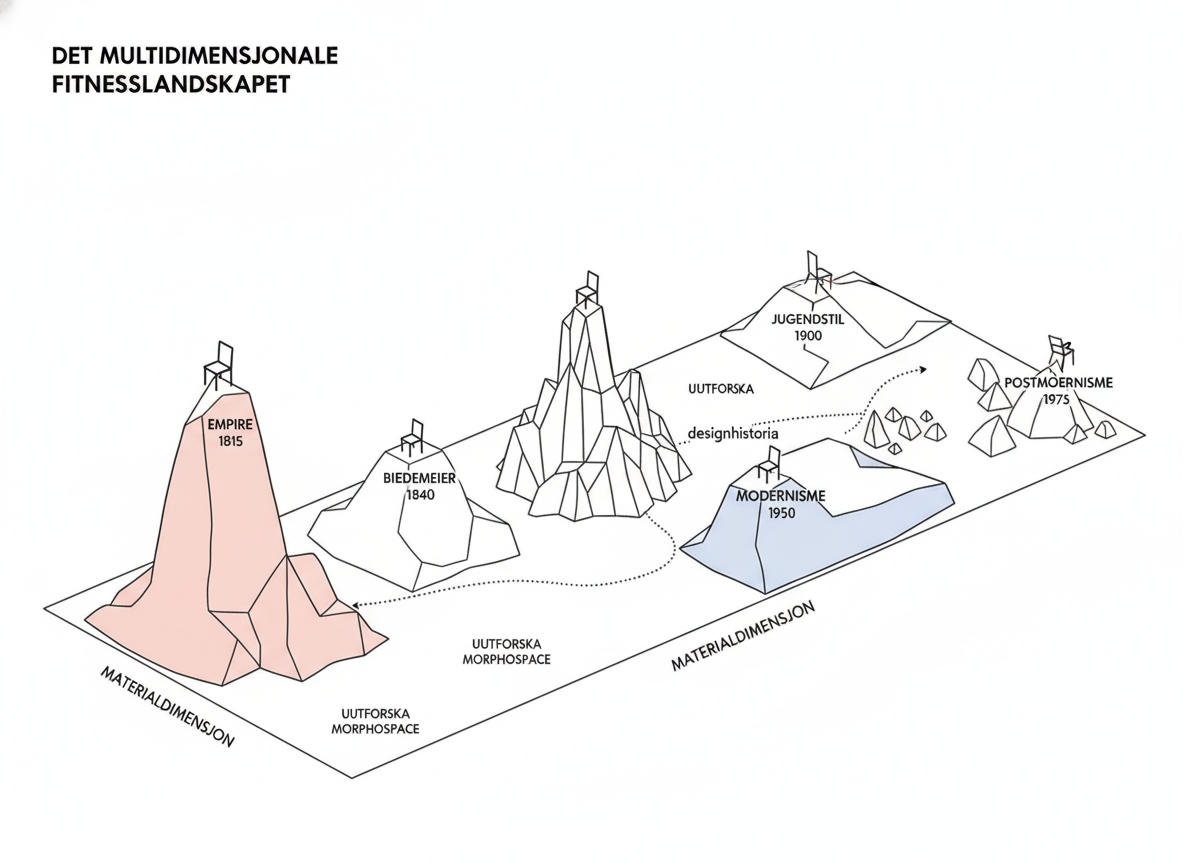
\includegraphics[width=\columnwidth]{ill03_fitnesslandskap.png}
  \caption{Det multidimensjonale fitnesslandskapet. Kvar topp representerer ein stilperiode (lokalt optimum). Barrokk er hoegast (mest materielt intensiv); postmodernisme er flatast (mest materiellt egalitaer). Materialdimensjonen og kulturdimensjonen definerer terrenget.}
  \label{fig:fitnesslandskap}
\end{figure}

\subsection{Distribuert kognisjon}

\begin{figure}[!ht]
  \centering
  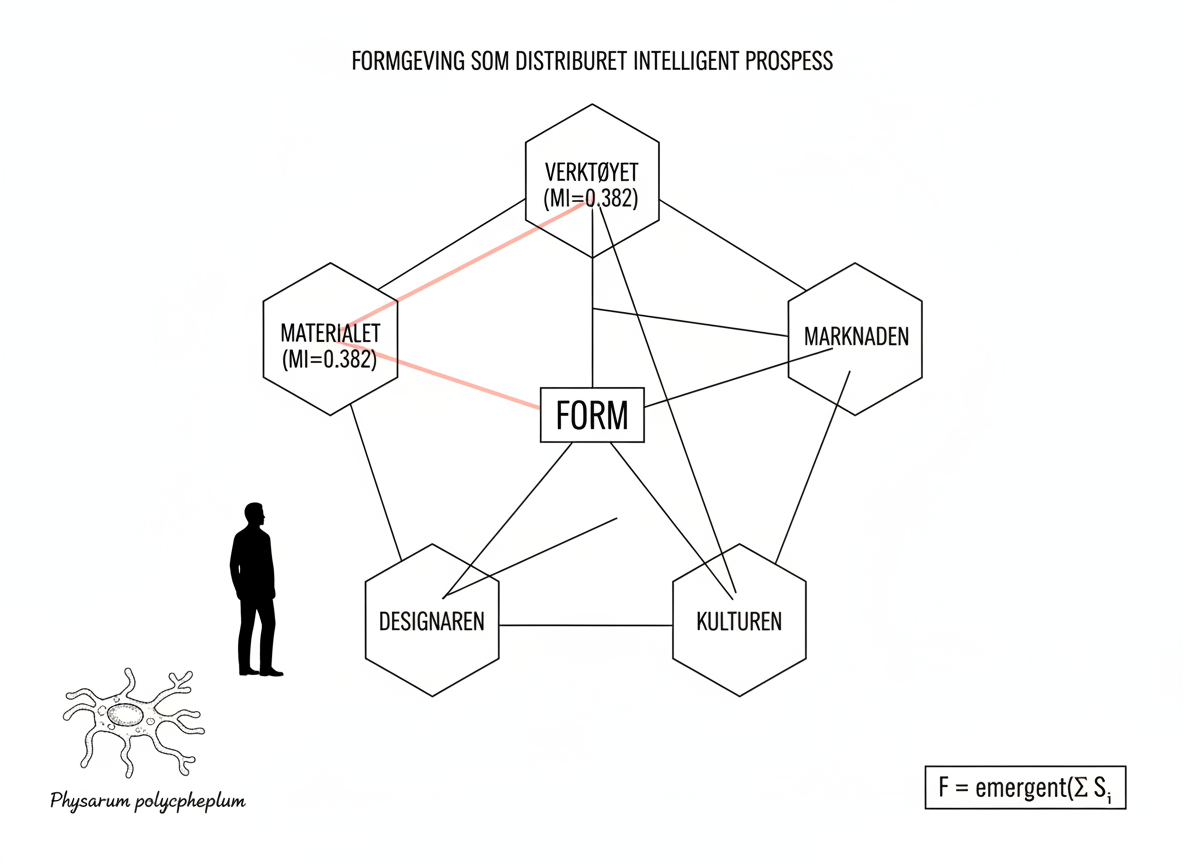
\includegraphics[width=\columnwidth]{ill04_distribuert.png}
  \caption{Formgjeving som distribuert intelligent prosess. Materialet (MI=0,382), verktoyeet (MI=0,382), designaren, marknaden og kulturen utover alle agentur. Forma er emergent, ikkje dedusert. Physarum-analogi nedst til venstre.}
  \label{fig:distribuert}
\end{figure}

\citet{hutchins1995} viste i \textit{Cognition in the Wild} at navigasjonen av eit marinefartøy ikkje er lokalisert i hovudet til éin navigatør, men distribuert over eit nettverk av menneske, instrument, kartverk og rutinar. \citet{clark2008} formulerte den utvida kognisjonshypotesen: kognitive prosessar strekkjer seg utover hjernen og inn i kroppen og miljøet. \citet{levin2019} utvida dette til ein generell teori om kognisjon på alle skalaer, frå einskildceller til organismar, med omgrepet ``kognitiv lyskjegle'' (\textit{cognitive lightcone}): det rommet av framtidige tilstandar eit system kan modellere og navigere mot.

Den mest slåande empiriske illustrasjonen av distribuert kognisjon i eit ikkje-neuralt substrat kjem frå \citet{nakagaki2000}, som demonstrerte at slimsoppen \textit{Physarum polycephalum} løyser labyrintar optimalt. Slimsoppen har ingen hjerne, ingen nevron, inga sentralisert styring. Likevel navigerer han mot mat gjennom ein distribuert algoritme der kvar del av organismen responderer lokalt på næringsgradientar. Resultatet er ei global løysing som tilnærmar seg det kortaste stieproblemet.

I FFF tyder dette at formgjeving ikkje er ein reint mental prosess lokalisert i hovudet til formgjevaren. Materialet ``veit'' kva det toler: eik sprekk langs medmargen, stål bøyer seg elastisk, plast flyt under varme. Verktøyet avgrensar formrommet: ein dreiebenk produserer rotasjonssymmetriske former, ei CNC-maskin produserer former definerte av G-kode. Marknaden selekterer: ein stol som er for dyr, for tung eller for stilistisk framand overlever ikkje.

Omgrepet ``kognitiv lyskjegle'' \citep{levin2019} er særleg produktivt. Ein handverkar som arbeider med eik har ein lyskjegle avgrensa av materialet sine mekaniske eigenskapar, verktøyet si rekkjevidde, og sin eigen erfaringshorisont. Ein industridesignar med tilgang til parametrisk programvare, CNC-fresing og 50 ulike polymerar har ein radikalt vidare lyskjegle. Det er ikkje at den eine er smartare enn den andre; det er at det distribuerte systemet av designar-verktøy-materiale-marknad har ulik kognitiv rekkjevidde. \citet{sennett2008} skildra den intime forhandlinga mellom handverkar og materiale som ein dialog: materialet motset seg, handverkaren responderer, og forma veks fram gjennom ei iterativ forhandling der ingen av partane har full kontroll. FFF formaliserer denne intuisjonen: forma er eit emergent resultat av distribuert kognisjon i eit agentialt nettverk.

\subsection{Utforsking og utnytting}

Avveginga mellom \textbf{exploration} og \textbf{exploitation} er formalisert i forsterkingslæring \citep{sutton2018} og i paleontologien som \textbf{punctuated equilibrium} \citep{eldredge1972}. Problemet er universelt: eit system som berre utforskar finn aldri ro; eit system som berre utnyttar vert fanga i eit lokalt optimum og overlever ikkje eit landskapsskifte.

Designhistoria vekslar mellom desse to fasane: lange periodar med utnytting der forma konvergerer, avbrotne av raske utforskingsfasar utløyste av teknologiske eller geopolitiske sjokk. STOLAR-dataa gjer det mogleg å kvantifisere denne dynamikken med entropi.

\textbf{Mahognimonopolet som ekstrem utnytting.} I perioden 1825--1849 er 100\,\% av V\&A-stolane i datasettet laga med mahogni som primærmateriale. Shannon-entropien for materialar i denne perioden er nær minimum. Formrommet er sterkt innsnevra: materiallandskapet har kollapsa til eitt einaste toppunkt. Dette er utnytting driven til ytterpunktet, ein monokultur i materiell forstand. \citet{anderson1995} dokumenterer korleis det britiske imperiet organiserte heile forsyningskjeder frå Honduras og Jamaica til London for å mate denne etterspurnaden. Mahognien var ikkje vald for funksjonelle grunnar (eik eller valnøtt ville bore ein sitjande kropp like godt), men for ein konstellasjon av affordansar (fin korntekstur, evne til å ta politur), statusmarkørar (eksotisk opphav, høg pris) og industrielle fordelar (standardiserte dimensjonar frå kolonialsagbruk).

\textbf{Industrialiseringa som utforskingssjokk.} Når dampkraft, stålproduksjon og nye limtypar vert tilgjengelege etter 1850, eksploderer formrommet. Entropien stig bratt. Nye materialar opnar nye regionar av landskapet. Michael Thonet sin formbøyingsteknologi, dokumentert av \citet{thonet1976}, tillét masseprodukt stol nr.~14 i bøkt bøketre, ein radikal utforsking av ein tidlegare utilgjengeleg region. Entropitalet dokumenterer sjokket: frå 1800-talet til 1900-talet stig $H'$ frå omlag 3,5 til 5,07 bits, den høgste verdien i heile datasettet. Industrialiseringa er ikkje berre eit skifte i produksjonsmetode; det er eit fundamentalt landskapsskifte som opnar heilt nye dalar og toppunkt.

\textbf{Entropimønsteret.} Det overordna mønsteret er ein monotont stigande entropikurve (figur~\ref{fig:entropi}), men med fleire faseskifte: ein trappetrinnsauke rundt 1600 (kolonialhandel), eit platå på 1700-talet (utnytting av det koloniale repertoaret), ein ny trappetrinnsauke rundt 1850 (industrialisering), og ein jamn vekst gjennom 1900-talet (syntetiske materialar). Kvar fase svarar til eit skifte mellom utforsking og utnytting, og kvar overgang svarar til eit landskapsskifte.

\begin{figure}[!ht]
  \centering
  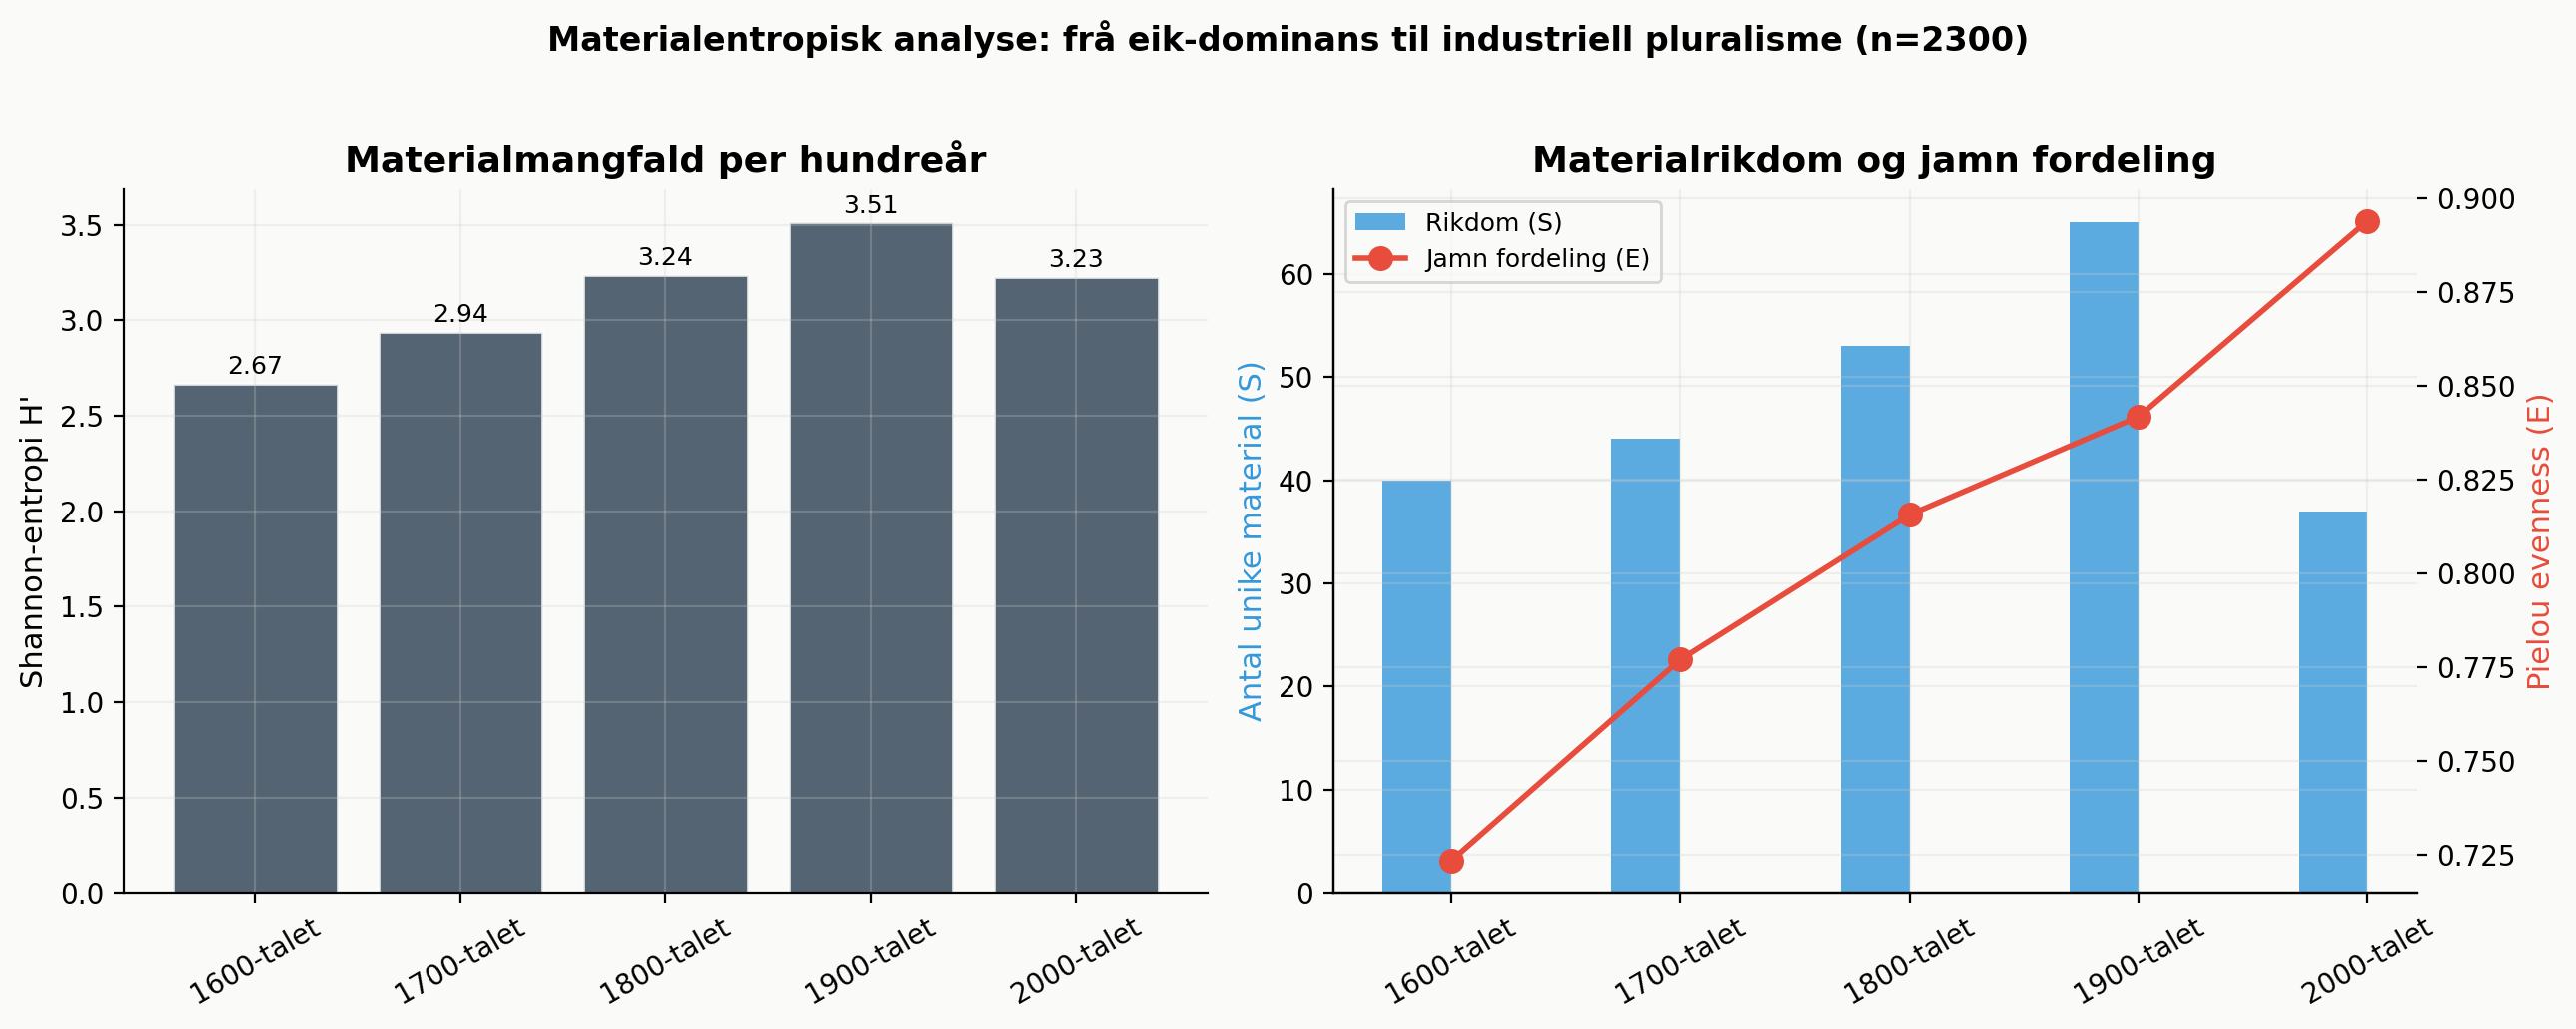
\includegraphics[width=\columnwidth]{07_material_entropy.png}
  \caption{Shannon-entropi for materialar over tid ($H'$, bits). Monotont stigande, med tre tydelege faseskifte som svarar til kolonialhandel, industrialisering og syntetisk revolusjon.}
  \label{fig:entropi}
\end{figure}

\subsection{Affordanse}

\citet{gibson1977} definerte \textbf{affordanse} som dei handlingsmoglegheitene eit miljø tilbyr ein organisme. \citet{pye1968} skilde mellom ``the workmanship of risk'' og ``the workmanship of certainty''. \citet{ingold2013} utvida affordanseomgrepet til materialar: eit materiale tilbyr ikkje berre moglegheiter, det motsetter seg og kanaliserer. I FFF yter kvart materiale ei distinkt form for tilbod og motstand, ein affordanse som fysisk kanaliserer bestemte geometriar og stengjer andre ute.

\begin{figure}[!ht]
  \centering
  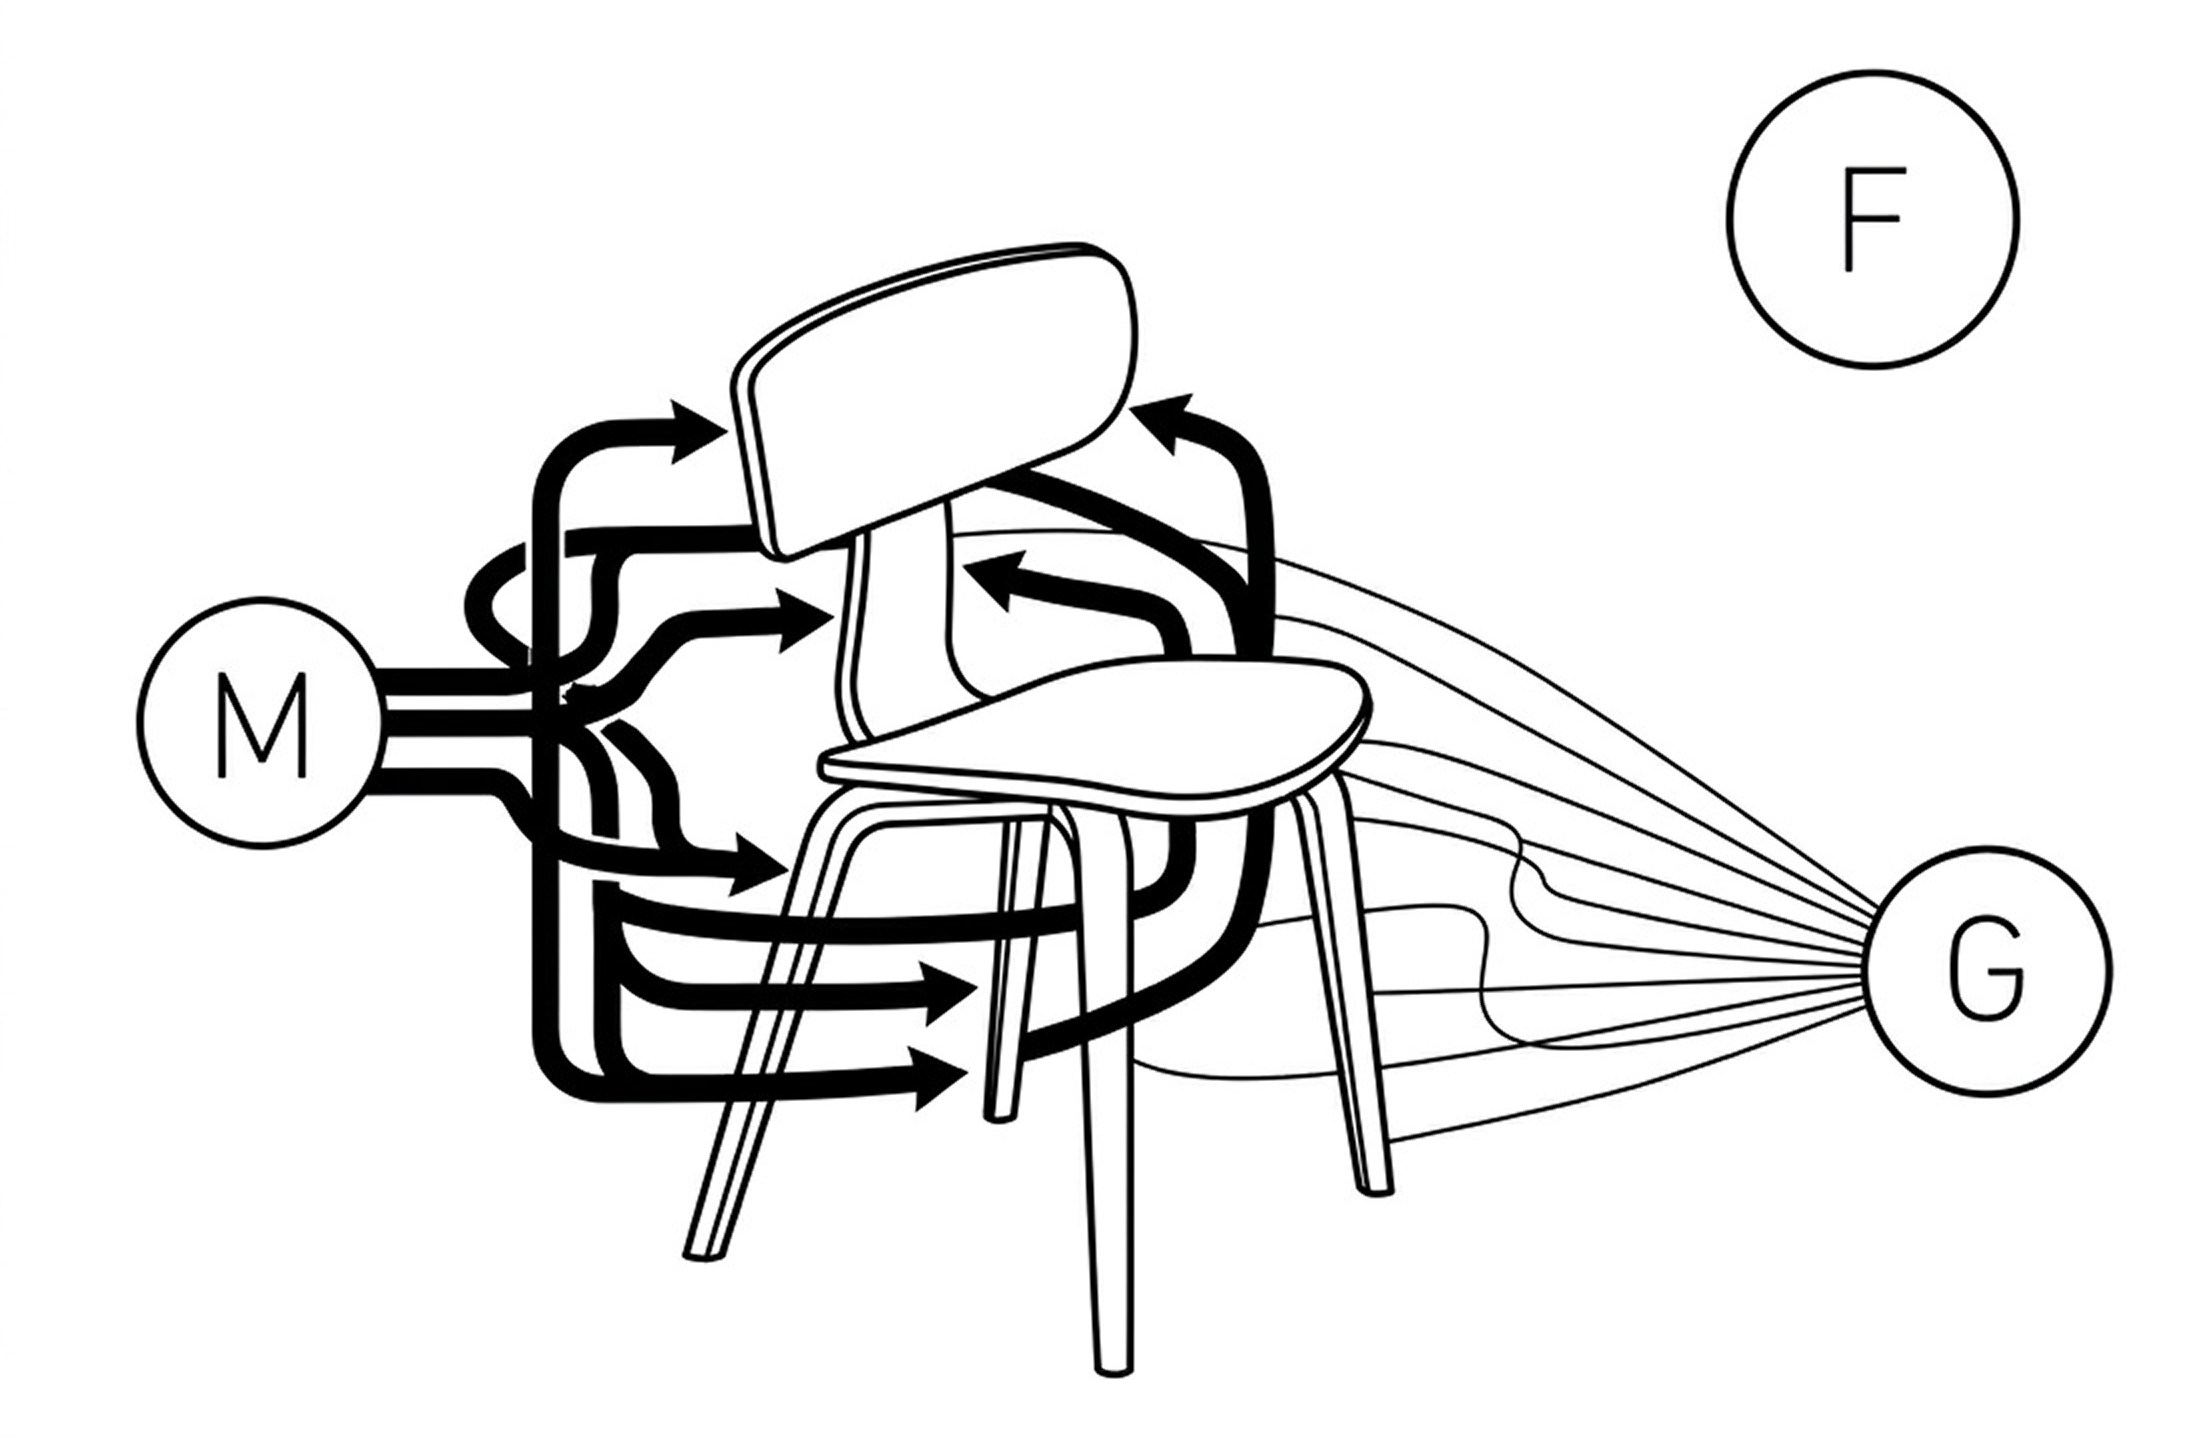
\includegraphics[width=\columnwidth]{teikn_funksjoner.png}
  \caption{Kreftene bak ein stol: materialet (M), funksjonen (F) og geografien (G) utover alle seleksjonstrykk paa den endelege forma. Pilane viser korleis kreftene kanaliserer konstruksjonen.}
  \label{fig:funksjoner}
\end{figure}

STOLAR-dataa gjev den fyrste kvantitative dokumentasjonen av denne kanaliseringseffekten. $H/W$-ratioen (høgde delt på breidde) varierer systematisk mellom materialgrupper:

\begin{itemize}
  \item \textbf{Stål:} $H/W = 1{,}29$ (SD = 0,31). Stål tillét slanke, vertikale konstruksjonar med tynt tverrsnitt. Materialet si høge strekkfastleik gjer det mogleg å bere last med minimalt volum.
  \item \textbf{Bjørk:} $H/W = 1{,}81$ (SD = 0,44). Bjørk krev breiare tverrsnitt for å bere same last, og tradisjonell tappekonstruksjon favoriserer høge, smale proporsjonar.
  \item \textbf{Plast:} $H/W = 1{,}22$ (SD = 0,28). Sprøytestøypte plastformer tenderer mot kompakte, organiske geometriar utan tradisjonelt understell.
  \item \textbf{Mahogni:} $H/W = 1{,}55$ (SD = 0,35). Mahogni ligg mellom stål og bjørk, noko som reflekterer materialet si evne til å ta både slanke og massive former.
\end{itemize}

Skilnaden mellom ytterpunkta (stål 1,29 mot bjørk 1,81) gjev Cohen's $d = 0{,}51$, ein medels effektstorleik. Materialet er altså ikkje berre ein overflate som dekkjer ein funksjonelt diktert struktur; det er ein aktiv formgjevande kraft som systematisk kanaliserer geometrien. $\chi^2$-testen for assosiasjon mellom materialgruppe og proporsjonsklasse gjev $\chi^2 = 633{,}8$ ($p < 0{,}001$), noko som inneber at nullhypotesen om uavhengigheit mellom materiale og form kan avvisast med overveldande konfidens.

\begin{figure}[!ht]
  \centering
  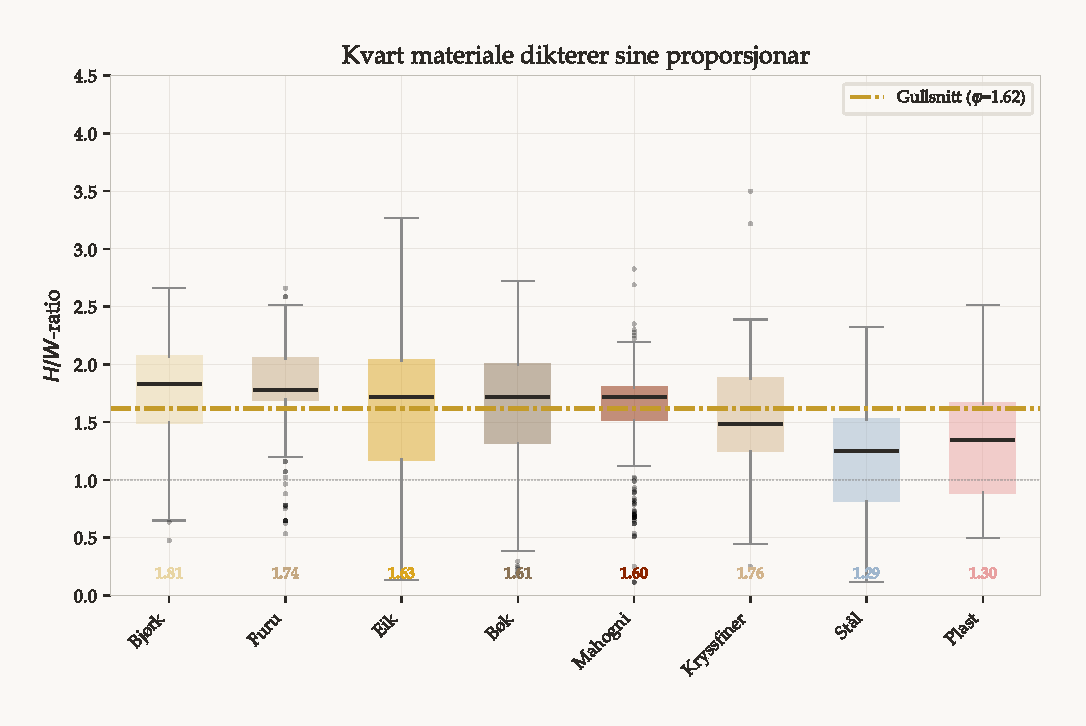
\includegraphics[width=\columnwidth]{fig11_hw_per_material.pdf}
  \caption{$H/W$-ratio per materialgruppe. Kvart materiale kanaliserer ein distinkt proporsjonsregion.}
  \label{fig:hwmaterial}
\end{figure}

\citet{ashby2013} tilbaud ein systematikk for materialval i produktdesign, men utan empirisk evidens frå faktiske historiske objekt. \citet{manzini1986} argumenterte for at materialar er ``invensjonens stoff'', men utan kvantitative data. STOLAR-datasettet gjev den empiriske grunngjevinga som desse teoretikarane mangla: materialet kanaliserer form, og denne kanaliseringa er målbar.

\subsection{Morforom}

\citet{raup1966} introduserte \textbf{morphospace}: det teoretiske rommet av alle moglege former ein biologisk struktur kan innta. Raup studerte snigelskal og viste at av dei matematisk moglege kombinasjonane av spiralparametrar, er berre ein liten region faktisk realisert i naturen. Dei tome regionane er like informative som dei fylte: dei fortel kva former som er fysisk, mekanisk eller biologisk umoglege.

I FFF er formrommet analogt: totaliteten av alle moglege geometriske, materielle og operasjonelle tilstandar ein stol kan innta. Dei fire dimensjonane (høgde, breidde, djupn, setehøgde), kombinert med 76 materialar og 38 teknikkar, spenner opp eit formrom med enormt mange teoretiske kombinasjonar. Men dei realiserte kombinasjonane okkuperer berre ein liten del av dette rommet.

Dei tome regionane fortel oss kva former som er umoglege gjeve dei gjeldande seleksjonstrykka. Det finst ingen stolar i datasettet som kombinerer plast med tradisjonell tapping, fordi materialet ikkje tillèt det. Det finst ingen stolar som kombinerer granitt med formbøying. Det finst nesten ingen stolar under 50 cm høgde (med unnatak av barnestolar), fordi ergonomien set ei nedre grense. Desse fråvera er ikkje tilfeldige; dei er systematiske, og dei reflekterer dei same seleksjonstrykka som FFF postulerer.

Det kanskje mest interessante funnet er dei diakrone skifta i okkupert formrom. I mellomalderen er det realiserte formrommet ein liten, kompakt klynge i hjørnet av det teoretiske rommet: få materialar, få teknikkar, høge og smale proporsjonar. Over tid ekspanderer den okkuperte regionen i alle retningar samstundes som han fragmenterer seg i underklynger, éin for kvar materialregime. Denne ekspansjonen er ikkje kontinuerleg; han skjer i diskrete sprang som svarar til dei same faseskifta som entropikurva dokumenterer. Formrommet puster: det utvider seg ved kvart landskapsskifte og kontraherer delvis i utnyttingsfasar.

\subsection{Sullivan som degenerert spesialtilfelle}

``Form follows function'' er logisk gyldig berre når alle seleksjonstrykk utanom funksjon er eksakt lik null. Fellesinformasjonsanalysen (figur~\ref{fig:mi}) syner at funksjon ber \emph{null} informasjon om stilperiode (MI = 0,000 bits), medan proporsjonar ber 2,072 bits, tid 1,546 bits, og materiale 1,456 bits. Funksjonalismen er eit degenerert spesialtilfelle.

Meir presist: i eit system der alle stolar deler same funksjon (å bere ein sitjande kropp), er funksjonen ein konstant. Ein konstant variabel har null entropi og kan per definisjon ikkje bere informasjon om nokon annan variabel. Sullivan sitt aksiom kollapsar ikkje fordi det er feil i ein abstrakt, logisk forstand, men fordi det er empirisk tomt. Det predikerer ein tilstand (funksjonell konvergens) som aldri er observert i datamaterialet. Aksiomet er ikkje falskt; det er degenerert, gyldig berre i eit vakuum av seleksjonstrykk som aldri har eksistert i den reelle verda.

\begin{figure}[!ht]
  \centering
  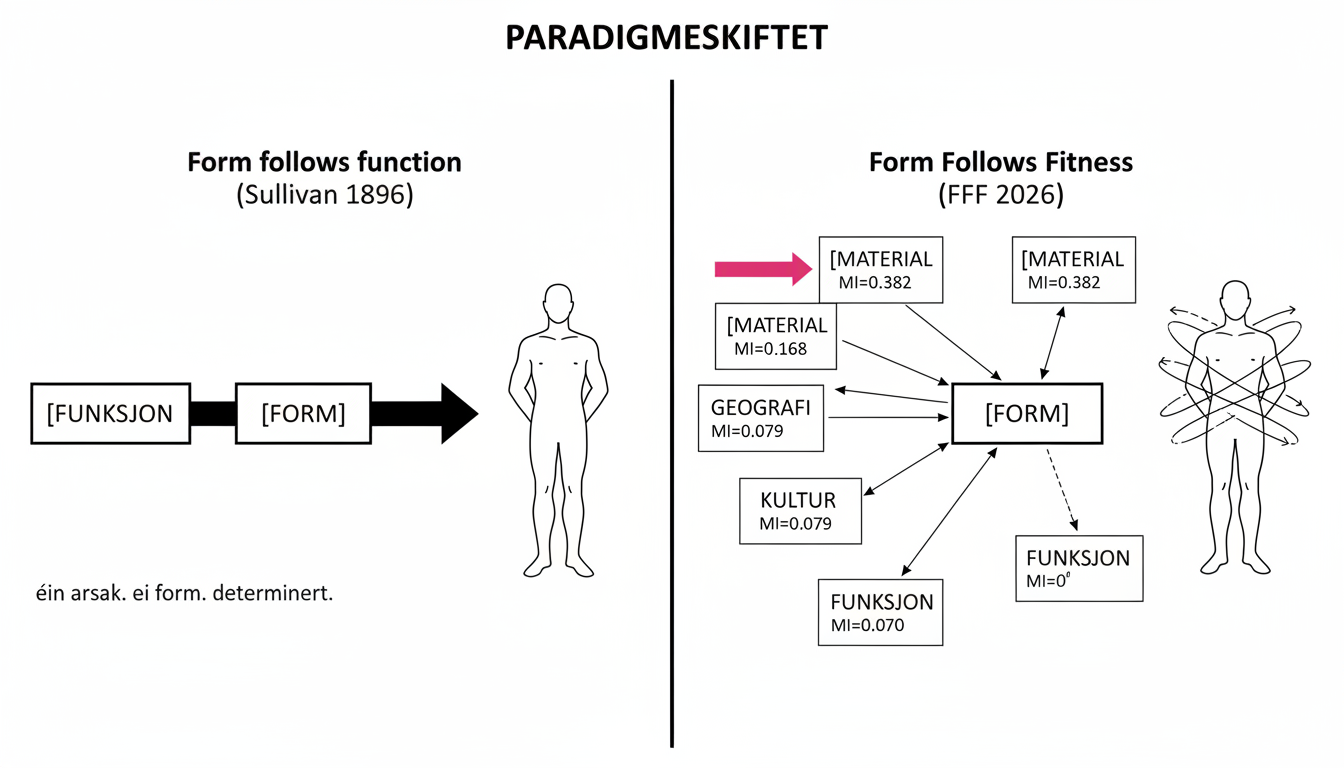
\includegraphics[width=\columnwidth]{ill05_paradigme.png}
  \caption{Paradigmeskiftet: fraa deterministisk funksjonalisme (ein aksial, ein form) til Form Follows Fitness (fleirdimensjonalt fitnesslandskap med fleire lokale optimum). Sullivan sitt aksiom er eit 1D-spesialtilfelle av eit $n$-dimensjonalt rammeverk.}
  \label{fig:paradigme}
\end{figure}

\begin{figure}[!ht]
  \centering
  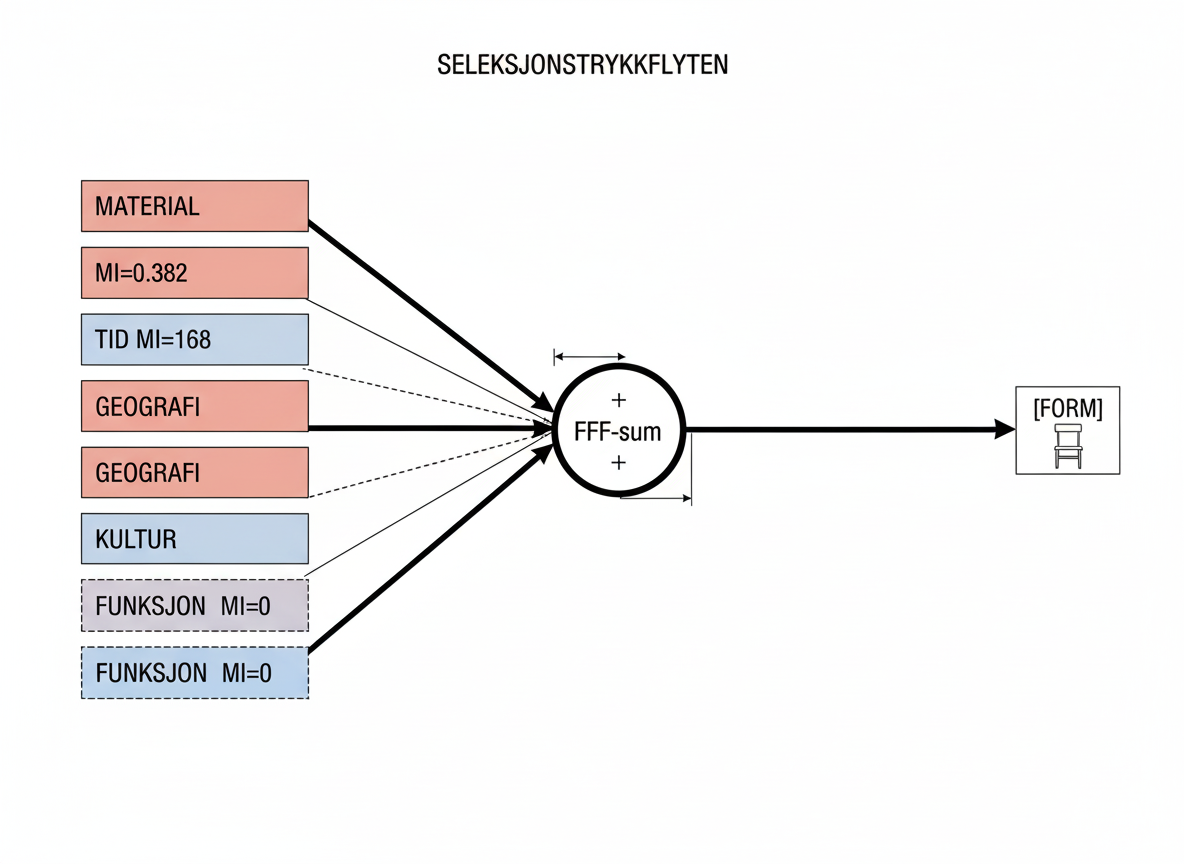
\includegraphics[width=\columnwidth]{ill01_seleksjonstrykk.png}
  \caption{Seleksjonstrykk-flyten: materiale, tid, geografi, kultur og funksjon bidreg alle med ulike MI-verdiar til den endelege forma. Funksjon (MI=0) er den svakaste inngangen.}
  \label{fig:seleksjon}
\end{figure}


% ================================================================
\section{Metode og datamateriale}

\subsection{Datainnsamling}

STOLAR-databasen vart bygd frå to kjelder. NMK-dataa ($n \approx 700$) vart henta frå Digitalt Museum (DiMu) sitt API og supplerte med manuell kontroll. V\&A-dataa ($n \approx 1\,600$) vart henta frå museet sitt opne API. Alle postar vart harmoniserte til eit felles skjema. Etter filtrering (ekskludering av postar utan dimensjonsdata, duplikat og feilregistreringar) gjensto 2\,284 objekt. Datafangsten vart gjennomført i fleire rundar mellom 2024 og 2025, med systematisk kvalitetskontroll mellom kvar runde.

Harmoniseringa var ikkje triviell. NMK og V\&A nyttar ulike katalogsystem, ulike materialterminologiar og ulike dimensjonskonvensjonar. NMK oppgjev dimensjonar som ``H x B x D'', V\&A som ``Height, Width, Depth'' med varierande einingar. Materiallistene måtte normaliserast frå fritekst (``ebonised beechwood with cane seat and gilt bronze mounts'') til standardiserte kategoriar.

\subsection{Variablar}

\textbf{Dimensjonar:} Høgde, breidde, djupn, setehøgde (i cm). \textbf{Materialar:} Kommaseparerte lister, koda til 30 binære variablar for maskinlæring. \textbf{Teknikkar:} Kommaseparerte lister av konstruksjonsteknikkar. \textbf{Metadata:} Produksjonsår, stilperiode, nasjonalitet, museum.

\subsection{Materialkoding: 27 binære variablar}

Eit sentralt metodisk val var å transformere materialteksten frå fritekstformat til binære indikatorvariablar. Råteksten i museumspostane er heterogen og inkonsistent: ``oak and walnut with silk upholstery'', ``mahogany, brass, leather'', ``bjørk, furu, skinn''. Å bruke slike tekststrenger direkte i statistiske modellar ville krevje avansert naturleg språkprosessering og ville introdusere støy frå skrivevariasjon, språkskilnader og katalogiseringspraksisar.

I staden identifiserte eg 27 materialkategoriar som dekkjer $> 95\,\%$ av alle materialoppføringar i datasettet, og koda kvar stol som ein binær vektor $\mathbf{m} \in \{0, 1\}^{27}$. Ein stol i ``mahogni og silke'' får $m_{\text{mahogni}} = 1$, $m_{\text{silke}} = 1$, og alle andre $m_i = 0$. Denne tilnærminga har tre fordelar: (1) ho er reproduserbar, (2) ho tillèt standard statistiske metodar, og (3) ho bevarer kombinasjonsinformasjon.

Tilnærminga har også avgrensingar. Ho skil ikkje mellom primære og sekundære materialar (ein stol ``i eik med mahognifanér'' og ein stol ``i mahogni med eikesarg'' får same vektor dersom begge materiala er registrerte). Ho fangar ikkje proporsjonane mellom materiala. Og ho er avhengig av at museumspostane er korrekt og komplett. Trass i desse avgrensingane viste $\chi^2$-testen at assosiasjonane mellom dei binære materialvariablane og formvariablane er statistisk signifikante: $\chi^2 = 633{,}8$ ($p < 0{,}001$, $df = 216$).

\subsection{Informasjonsteori: MI-berekning}

Fellesinformasjon (Mutual Information, MI) vart brukt som hovudmål for assosiasjon mellom variablar. MI er definert som
\[
  \text{MI}(X;Y) = \sum_{x \in X} \sum_{y \in Y} p(x,y) \log_2 \frac{p(x,y)}{p(x)\,p(y)}.
\]
MI måler kor mange bits informasjon kjennskap til variabel $X$ gjev om variabel $Y$ \citep{cover2006}. I motsetnad til korrelasjonskoeffisientar fangar MI også ikkje-lineære samanhengar, noko som er viktig fordi samanhengen mellom til dømes materiale og stilperiode er kategorisk og ikkje lineær.

MI vart berekna mellom stilperiode og kvar av følgjande variablar: proporsjonar (diskretiserte $H/W$-ratio), tid (hundreår), materiale (dei 27 binære variablane aggregerte), teknikk, nasjonalitet og funksjon. Resultata (figur~\ref{fig:mi}) viser at proporsjonar ber mest informasjon om stilperiode (MI = 2,072 bits), følgd av tid (1,546 bits) og materiale (1,456 bits). Funksjon ber MI = 0,000 bits, fordi funksjonen er invariant over heile datasettet.

\subsection{Statistiske metodar}

\begin{itemize}
  \item \textbf{Informasjonsteori:} Shannon-entropi ($H'$) og Pielou-jamnheit ($J'$) for å måle material- og teknikkmangfald over tid \citep{shannon1948, pielou1966, magurran2004}.
  \item \textbf{Klassifikasjon:} Random Forest \citep{breiman2001} med 100 trær og 5-faldig stratifisert kryssvalidering for å predikere stilperiode, nasjonalitet og hundreår.
  \item \textbf{Avstandsmål:} Jaccard-avstand for materialsamanlikning mellom museum, berekna som $J = 1 - |A \cap B| / |A \cup B|$.
  \item \textbf{Effektstorleik:} Cohen's $d$ for dimensjonsskilnader mellom grupper.
  \item \textbf{Assosiasjonstestar:} $\chi^2$-test for uavhengigheit mellom kategoriske variablar.
\end{itemize}

\subsection{Avgrensingar}

Fire viktige atterhald: (1) Variablane er grove (fire lineære dimensjonar, ikkje fullstendig 3D-geometri). Ein stol sin skulpturelle kvalitet, kurvatur og detaljerikdom er ikkje fanga. (2) V\&A dominerer datasettet med 70,6\,\% av observasjonane, noko som kan introdusere ein museumssamlarbias. (3) Berre 22,9\,\% av objekta har stilmerke; alle klassifikasjonsresultat for stilperiode er difor baserte på dette delsettet. (4) Museumssamlingar er ikkje representative populasjonar; dei er kuraterte utval som favoriserer det sjeldne, det vakre og det historisk viktige. Kvardagsmøblar er underrepresenterte.

Trass i desse avgrensingane er beviskjeda kumulativ og konvergent: fire uavhengige analysar peikar mot same konklusjon. Sjølv om kvar einskild analyse har sine avgrensingar, er det usannsynleg at alle fire peikar i same retning ved tilfelde.


% ================================================================
\section{Dei fire artiklane}

\subsection{Artikkel I: Materialar som geopolitisk historie}

Den fyrste artikkelen introduserer \textbf{materialkurveanalyse} som metode for å lese materialhistorie kvantitativt. Hovudfunnet er at materialpaletten i europeisk stoldesign ikkje ekspanderer jamnt, men i diskrete regimeskifte som svarar til geopolitiske omveltingar.

Shannon-entropien for materialar stig monotont frå $H' = 1{,}0$ bits (1200-talet, 2 materialar) til $H' = 5{,}07$ bits (1900-talet, 65 materialar). Entropien er ikkje berre eit mål på mangfald; ho er eit mål på uføreseielegheita til materialet i ein tilfeldig vald stol. I mellomalderen kan ein gjette materialet med stor sannsyn (bjørk eller eik); i det tjuande hundreåret er materialet nær uføreseieleg.

Analysen avdekkjer tre materialregime:

\begin{enumerate}
  \item \textbf{Det lokale treregimet} (1200--1500): bjørk, furu, eik. $H' < 2$ bits. Materialpaletten er avgrensa til det som veks lokalt. Transport er dyrt og langsomt; materialar reiser ikkje langt.
  \item \textbf{Det koloniale handelsregimet} (1600--1800): mahogni dominerer med opp til 17,3\,\% i V\&A. Perioden 1825--1849 er eit ytterpunkt: 100\,\% av V\&A-stolane i denne perioden har mahogni som primærmateriale. Jaccard-avstanden mellom NMK og V\&A fell frå 1,0 til 0,47, noko som tyder at samlingane nærmar seg kvarandre i materialsamansetnad ettersom globale handelsvegar integrerer europeiske materialmarknader. \citet{wallerstein2004} sin verdsystemteori gjev det geopolitiske rammeverket: mahogni er ikkje eit designval, men eit imperielt infrastrukturprodukt.
  \item \textbf{Det industrielt-syntetiske regimet} (1900--2000): stål, kryssfiner, plast. Industrielle materialar når 32,3\,\% av alle registrerte materialar. Materialpaletten ekspanderer eksplosivt. \citet{heskett1980} dokumenterte korleis industriell design oppsto som ein ny profesjon nettopp fordi det nye materialrepertoaret kravde nye kompetansar.
\end{enumerate}

Artikkelen innfører omgrepet \textbf{materiell dobbeltheit}: konstruksjonar der berande kjernar er lokalt tre, medan fasaden er importert edelt materiale. Fenomenet toppar med 23,5\,\% av stolane på 1800-talet, noko som demonstrerer at materialet har ein dobbel funksjon: strukturell (å bere last) og semiotisk (å kommunisere status og tilhøyrsle).

\begin{figure}[!ht]
  \centering
  
\includegraphics[width=\columnwidth]{fig4_jaccard.pdf}
  \caption{Jaccard-avstand mellom NMK og V\&A over tid. Samlingane konvergerer i materialsamansetnad under det koloniale regimet.}
  \label{fig:jaccard}
\end{figure}

\subsection{Artikkel II: Produksjonsgeografi og formkonvergens}

Den andre artikkelen undersøkjer korleis geografi og tid påverkar form. Hovudfunnet er at forma driftar systematisk under geografisk og teknologisk påverknad, og at denne drifta er inkompatibel med funksjonsdeterminisme.

Gjennomsnittleg høgde fell frå 94,7 cm (1200-talet) til 73,1 cm (2000-talet), ein reduksjon på 22,8\,\%. Denne drifta er ikkje forklart av endringar i menneskekroppen (europeisk gjennomsnittshøgde auka i same periode). Ho er konsekvent 18--40 cm under Le Corbusier sin Modulor-prediksjon \citep{lecorbusier1950}. Modulor-avviket er systematisk negativt i alle periodar, noko som tyder at stolar er konsekvent lågare enn det ein ergonomisk-funksjonalistisk modell predikerer.

$H/W$-ratioen driftar frå 1,68 (1200-talet) til 1,37 (2000-talet), vekk frå gullsnittet ($\varphi = 1{,}618$) og mot meir kompakte proporsjonar. Denne drifta reflekterer overgangen frå tronliknande, vertikale stolar (der høgda kommuniserer status) til låge, horisontale sitjemøbel (der komfort og materiell effektivitet er viktigare seleksjonskriterium).

\begin{figure}[!ht]
  \centering
  
\includegraphics[width=\columnwidth]{fig9_nmk_va_hogde.pdf}
  \caption{Gjennomsnittleg høgde i NMK vs.\ V\&A over tid. NMK-stolar er systematisk høgare i tidlege periodar, men konvergerer med V\&A etter industrialiseringa.}
  \label{fig:nmk_va}
\end{figure}

NMK-stolar er systematisk høgare enn V\&A-stolar i tidlege periodar ($\Delta = +24{,}6$ cm i 1600-talets gjennomsnitt), men skilnaden konvergerer mot null etter industrialiseringa, for deretter å divergere igjen i skandinavisk modernisme. Denne konvergens-divergens-syklusen er eit direkte uttrykk for landskapsdynamikken: når same materialar og teknikkar vert tilgjengelege i begge land (kolonialhandel, industrialisering), konvergerer formene; når lokale designtradisjonar vert kulturelt viktige (skandinavisk modernisme), divergerer dei igjen.

Estimert medianvekt fell frå 20,4 kg (mellomalder) til 6,8 kg (samtid), ein reduksjon med ein faktor 3. Denne vektreduksjonen reflekterer overgangen frå massivt tre til rørformer i stål og formpressa skjel i plast. Materialet endrar seg; forma følgjer materialet.

\subsection{Artikkel III: Form og tid}

Den tredje artikkelen brukar maskinlæring for å teste kva variablar som kodar stil. Hovudfunnet er at stilperiode er ein emergent eigenskap, ikkje ein kausal kategori: den vert best predikert av dei same variablane (dimensjonar og materialar) som FFF identifiserer som seleksjonstrykk.

Ein Random Forest-modell \citep{breiman2001} oppnår:

\begin{table}[!ht]
\centering
\begin{tabular}{@{}llc@{}}
\toprule
\textbf{Features} & \textbf{Mål} & \textbf{$F1$} \\
\midrule
Dimensjonar åleine & Stilperiode & 0,777 \\
Materialar åleine & Stilperiode & 0,678 \\
Dimensjonar + materialar & Stilperiode & 0,823 \\
Dimensjonar + materialar & Nasjonalitet & 0,721 \\
Dimensjonar + materialar & Hundreår & 0,776 \\
\bottomrule
\end{tabular}
\caption{Random Forest-resultat for ulike feature-sett og målvariablar. 5-faldig stratifisert kryssvalidering.}
\label{tab:rf}
\end{table}

Høgde er den viktigaste enkeltvariabelen (19,7\,\% feature importance), følgd av breidde (14,2\,\%) og djupn (11,8\,\%). Blant materiala er mahogni (7,3\,\%), eik (5,9\,\%) og stål (4,8\,\%) dei viktigaste. At dimensjonar åleine gjev $F1 = 0{,}777$ tyder at geometrien inneheld ein stor del av den historiske informasjonen, og at ein trena modell kan ``lese'' tidsepokar frå proporsjonar med vesentleg treffprosent.

Teknikk-entropien stig parallelt med materialentropien, frå 1,0 til 3,67 bits (figur~\ref{fig:teknikk}). Denne parallelliteten er venta under FFF: nye materialar opnar nye teknikkar, og nye teknikkar opnar nye regionar av formrommet.

\begin{figure}[!ht]
  \centering
  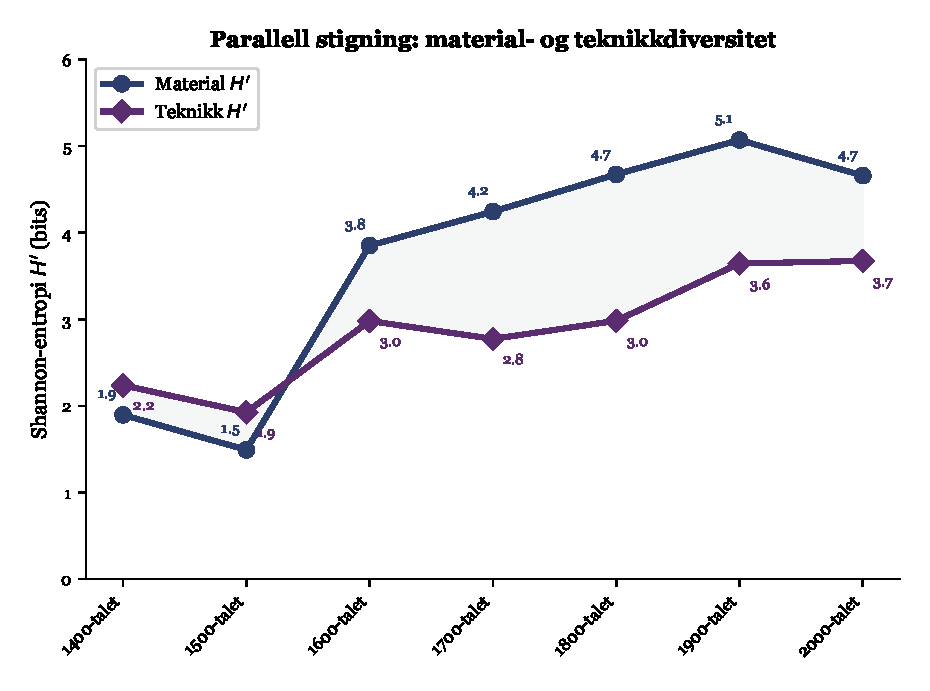
\includegraphics[width=\columnwidth]{fig8_teknikk_entropi.pdf}
  \caption{Shannon-entropi for teknikkar over tid. Parallelt forlaup med materialentropien.}
  \label{fig:teknikk}
\end{figure}

Den mest overraskande konklusjonen er at stilperiodar er emergente merkelappar, ikkje kausale kategoriar. Ein stol er ikkje ``barokk'' fordi han høyrer til barokken; han vert klassifisert som ``barokk'' fordi dimensjonane og materiala hans samsvarar med mønsteret til andre stolar produserte under same seleksjonstrykk. Stilmerket er ein konsekvens, ikkje ei årsak.

Fellesinformasjonsanalysen underbyggjer dette: proporsjonar ber MI = 2,072 bits om stilperiode, tid ber 1,546 bits, materiale ber 1,456 bits. Til saman ber desse variablane meir enn nok informasjon til å rekonstruere stilmerket. Stilperioden er redundant: ho er fullt ut kodet i dei fysiske eigenskapane.

\subsection{Artikkel IV: Form Follows Fitness}

Den fjerde artikkelen samlar åtte kumulative bevis, falsifiserer funksjonsdeterminismen, og formulerer FFF som eit testbart alternativ. Dei åtte bevisa er:

\begin{enumerate}
  \item Massiv formvariasjon under konstant funksjon.
  \item Monotont stigande materialentropi ($H' = 1{,}0 \rightarrow 5{,}07$ bits).
  \item Systematisk negativt Modulor-avvik ($-18$ til $-40$ cm).
  \item Konvergens-divergens-syklus mellom NMK og V\&A.
  \item Stilperiode best predikert av dimensjonar og materialar ($F1 = 0{,}823$), ikkje av funksjon.
  \item Funksjon ber null informasjon om stilperiode (MI = 0,000 bits).
  \item Proporsjonar ber 2,072 bits, meir enn nokon annan einskild variabel.
  \item Materialaffordanse kanaliserer geometri ($\chi^2 = 633{,}8$, $p < 0{,}001$).
\end{enumerate}

Artikkelen konkluderer med at funksjonalismen er eit degenerert spesialtilfelle, gyldig berre når alle seleksjonstrykk utanom funksjon er null. Sidan dette vilkåret aldri er oppfylt i den reelle verda, er aksiomet empirisk tomt. FFF erstattar det med eit rammeverk der form er selektert av eit fleirdimensjonalt tilpassingslandskap, og der funksjon berre er éin av mange krefter.


% ================================================================
\section{Syntese: frå fire artiklar til ein konklusjon}

\subsection{Beviskjeda}

Figur~\ref{fig:bevis} syner dei fire pilarane i beviskjeda.

\begin{figure}[!ht]
  \centering
  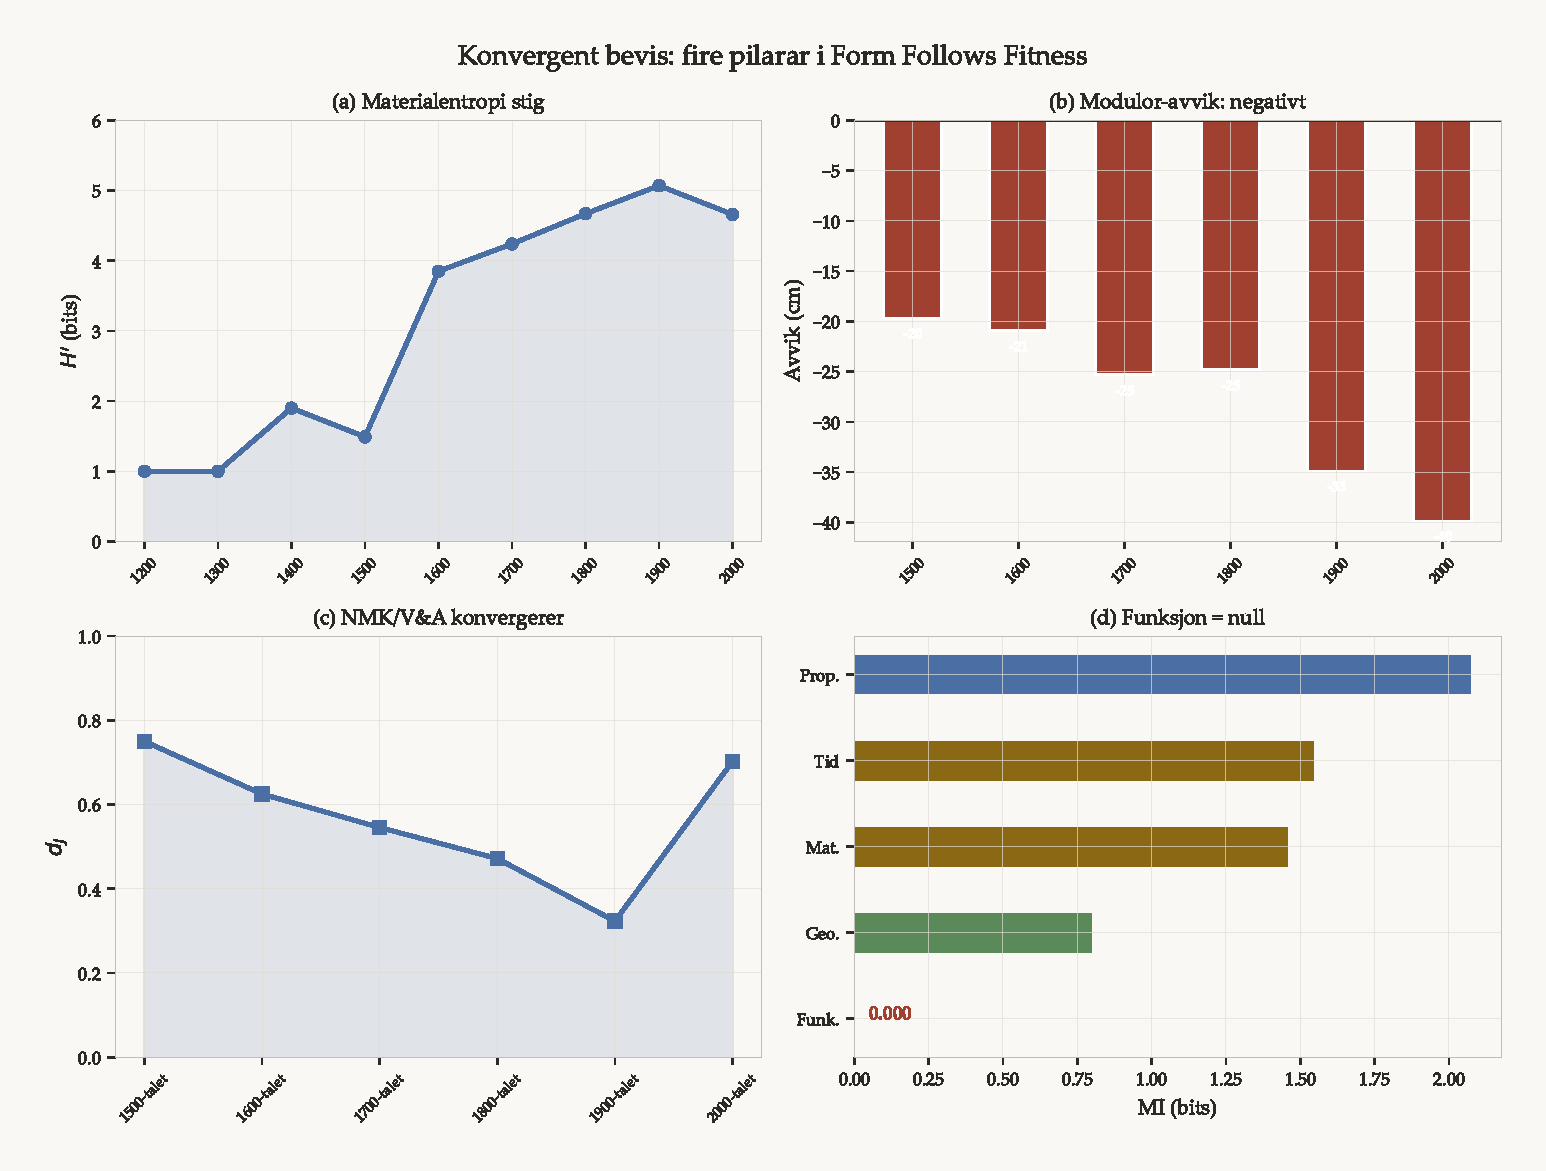
\includegraphics[width=\columnwidth]{fig16_beviskjede.pdf}
  \caption{Konvergent bevis: (a) materialentropi stig monotont, (b) Modulor-avviket er systematisk negativt, (c) Jaccard-avstanden mellom NMK og V\&A konvergerer, (d) funksjon ber null informasjon om stil.}
  \label{fig:bevis}
\end{figure}

Dei fire artiklane byggjer ein kumulativ beviskjede der kvar lekk styrkar dei andre:

\begin{itemize}
  \item \textbf{Artikkel~I} etablerer at materialar er agentiale substrat med eigne geopolitiske historier. Materialpaletten er ikkje ein nøytral meny designaren vel frå; det er eit historisk-geografisk produkt av handelsvegar, kolonialpolitikk og teknologisk infrastruktur. Shannon-entropien ($H' = 1{,}0 \rightarrow 5{,}07$ bits) dokumenterer at materialrommet ekspanderer i diskrete regimeskifte, ikkje jamnt.
  \item \textbf{Artikkel~II} viser at form driftar under geografisk og teknologisk påverknad, ikkje konvergerer mot funksjonelt optimum. Modulor-avviket ($-18$ til $-40$ cm) demonstrerer at stolar er konsekvent lågare enn det ein ergonomisk-funksjonalistisk modell predikerer. $H/W$-drifta (frå 1,68 til 1,37) viser at proporsjonane endrar seg systematisk, drive av materialskifte og kulturelle preferansar, ikkje av endringar i den sitjande kroppen.
  \item \textbf{Artikkel~III} demonstrerer at stilmerke er emergente restprodukt, ikkje årsaker. Ein Random Forest-modell predikerer stilperiode med $F1 = 0{,}823$ frå dimensjonar og materialar, men stilmerket åleine er den svakaste prediktoren for faktisk geometri. Fellesinformasjonsanalysen gjev det endelege svaret: proporsjonar ber MI = 2,072 bits om stilperiode, tid ber 1,546 bits, materiale ber 1,456 bits. Funksjon ber 0,000 bits.
  \item \textbf{Artikkel~IV} samlar bevisa og falsifiserer aksiomet. Funksjonalismen er eit degenerert spesialtilfelle, og FFF gjev eit empirisk testbart alternativ.
\end{itemize}

\subsection{Konvergens}

Styrken i beviskjeda ligg ikkje i noko einskild funn, men i konvergensen. Fire ulike analytiske tilnærmingar, frå informasjonsteori via maskinlæring til avstandsmål og effektstorleik, peikar mot same konklusjon. Denne konvergensen er vanskeleg å forklare om funksjonalismen var sann. Om form verkeleg følgde funksjon, skulle vi forvente (1) låg formvariasjon, (2) ingen systematisk materialeffekt på geometri, (3) at stilmerke er sterke prediktorar for geometri (fordi begge reflekterer funksjonen), og (4) at MI mellom funksjon og stilperiode er positiv. Alle fire prediksjonen vert falsifiserte.

\subsection{Paradigmeskifte}

\citet{kuhn1962} definerte eit paradigmeskifte som overgangen frå eitt sett av aksepterte normer til eit nytt. Kuhn identifiserte tre fasar: (1) normalvitskap under eit gjeldande paradigme, (2) anomali og krise når paradigmet ikkje lenger forklarer observasjonane, og (3) revolusjon når eit nytt paradigme erstattar det gamle. FFF oppfyller Kuhn sine kriterium på tre vis:

\begin{enumerate}
  \item \textbf{Anomali.} Funksjonalismen predikerer låg formvariasjon under konstant funksjon. Variasjonen er massiv. Gjennomsnittleg høgde varierer med ein faktor 1,6, estimert vekt med ein faktor 7, materialpaletten med 76 unike kategoriar. Denne variasjonen er ikkje støy; ho er systematisk og korrelert med identifiserbare seleksjonstrykk.
  \item \textbf{Krise.} Postfunksjonalismen har kritisert aksiomet i 50 år. \citet{sparke2004} dokumenterte designkultur som eit sosialt fenomen. Postmodernismen problematiserte universalisme. Men ingen har tilbode eit kvantitativt, testbart alternativ. Kritikken har vore kvalitativ, hermeneutisk og fragmentert. FFF konsoliderer denne kritikken i eit einskapeleg, kvantitativt rammeverk.
  \item \textbf{Nytt paradigme.} FFF subsumerer funksjonalismen som eit degenerert spesialtilfelle og gjev eit rammeverk som er empirisk falsifiserbart, kvantitativt og substratuavhengig. Det nye paradigmet forklarer alle observasjonane som det gamle ikkje kan forklare, samstundes som det inkluderer det gamle som eit grensetilefelle.
\end{enumerate}

\subsection{Fellesinformasjon som empirisk evidens}

Figur~\ref{fig:mi} oppsummerer kanskje det viktigaste einskilde funnet i heile avhandlinga. Fellesinformasjonsanalysen viser kor mange bits informasjon kvar variabel ber om stilperiode. Rekkjefølgja er:

\begin{enumerate}
  \item Proporsjonar (diskretisert $H/W$-ratio): MI = 2,072 bits (51,9\,\% av total).
  \item Tid (hundreår): MI = 1,546 bits (38,7\,\% av total).
  \item Materiale: MI = 1,456 bits (36,5\,\% av total).
  \item Teknikk: MI = 0,893 bits (22,4\,\% av total).
  \item Nasjonalitet: MI = 0,741 bits (18,6\,\% av total).
  \item Funksjon: MI = 0,000 bits (0,0\,\% av total).
\end{enumerate}

Funksjon ber bokstavleg talt null informasjon om stilperiode. Dette er ikkje eit statistisk artefakt; det er ein logisk nødvendigheit. Sidan alle stolar i datasettet deler same funksjon (å bere ein sitjande kropp), er funksjonen ein konstant, og ein konstant variabel har null entropi. Sullivan sitt aksiom er ikkje feil; det er tomt.

\subsection{Generalisering}

FFF er utvikla på stolar, men rammeverket er substratuavhengig. Same logiske struktur gjeld for alle gjenstandar som (1) har ein invariant funksjon, (2) varierer i form, og (3) er utsette for fleire samverkande seleksjonstrykk.

\textbf{Arkitektur.} Alle bygningar med same funksjon (bustad, kontor, kyrkje) varierer enormt i form. Ein gotisk katedral og ein betongbrutalistisk kyrkje deler funksjonen ``tilbedingsrom'', men divergerer radikalt i form. Materialet (stein vs.\ armert betong), teknologien (boge vs.\ utkraging), og den kulturelle konteksten (mellomalderleg kristendom vs.\ etterkrigssekularisme) utøver seleksjonstrykk som fullstendig overstyrer funksjonen.

\textbf{Typografi.} Alle skrifttypar med same funksjon (å representere bokstaven ``A'') varierer enormt i form. Garamond og Helvetica deler funksjonen, men divergerer i serif, x-høgde, kontrast og proporsjoner. Skriveteknologien (handskrift, blystøyping, fotosats, digital vektorgrafikk) endrar affordanserommet på same vis som materialet endrar stolens formrom.

\textbf{Bildesign.} Alle bilar med same funksjon (å transportere fire passasjerar) varierer enormt i form. Materialet (stål, aluminium, karbonfiber), produksjonsteknologien (handkaping, pressverk, robotsveising), regulatoriske krav (sikkerheit, utslepp), aerodynamiske seleksjonstrykk og kulturelle forventingar kanaliserer forma på same vis som i stoldesign.

\textbf{Biologisk morfogenese.} \citet{raup1966} sin morphospace-analyse viste at snigelskal varierer langs tre parameter, men at berre ein liten del av det teoretiske rommet er realisert. Dei same prinsippa gjeld: genetisk materiale (DNA), mekaniske krefter (vekst, tyngdekraft), og økologisk seleksjon kanaliserer forma. FFF er den kulturelle analogen til naturleg seleksjon.

I alle desse tilfella er forma ikkje dedusert frå funksjon, men selektert av eit landskap av samverkande krefter. FFF generaliserer frå stolar til alle estetiske og funksjonelle domene.

\citet{oxman2016} sitt omgrep \textbf{material ecology} definerer design som integrering av biologi, materialkunnskap og berekningsteknologi. FFF konvergerer mot same posisjon fraa ei anna retning: der Oxman argumenterer framover (korleis designpraksis \emph{bor} vere), argumenterer FFF bakover (korleis designhistoria \emph{faktisk} har vore). Begge landar paa same konklusjon: materialet er ein aktiv, formgjevande agent, ikkje eit passivt substrat.

Simon Conway Morris har argumentert for at konvergens er ei dominerande evolusjonaer kraft: gjeve like avgrensingar er evolusjonen ``bunden til aa snuble over'' like losningar. Analogen til design er direkte: stolar fraa ulike nasjonale tradisjonar konvergerer paa like dimensjonar fordi ergonomiske avgrensingar (menneskekroppen) fungerer som ein universell seleksjonskraft, akkurat som hydrodynamiske avgrensingar tvingar haiar og delfinar mot same kroppsfasong. ISO/TC 136 sine internasjonale mobelstandardar formaliserer denne konvergenskrafta regulatorisk.


% ================================================================
\section{Traktat for form}

\noindent\emph{Det deterministiske aksiomet har falle. Her byrjar tilpassinga.}

\bigskip

\noindent\textbf{1}\quad Formverda er alt som er tilfelle i det $n$-dimensjonale formrommet.

\medskip
\noindent\textbf{1.1}\quad Formrommet er totaliteten av alle moglege geometriske, materielle og operasjonelle tilstandar eit system, ein organisme eller ein gjenstand kan innta.

\medskip
\noindent\textbf{1.11}\quad Formrommet er ikkje metaforisk. For STOLAR-datasettet spenner det opp av fire dimensjonsvariablar, 27 binære materialvariablar og 38 teknikkvariablar. Totaliteten av moglege kombinasjonar er $> 10^{12}$. Dei realiserte kombinasjonane okkuperer ein forsvinnande liten del.

\medskip
\noindent\textbf{1.12}\quad Dei tome regionane av formrommet er like informative som dei fylte. Dei fortel kva former som er umoglege gjeve dei gjeldande seleksjonstrykka.

\medskip
\noindent\textbf{1.14}\quad Det deterministiske aksiomet frå det tjuande hundreåret, postulatet om at form let seg ufeilbarleg utleie direkte frå funksjon, er eit logisk usant bilete av røynda.

\medskip
\noindent\textbf{1.141}\quad Sullivan sin formulering ``form ever follows function'' er logisk gyldig berre under vilkåret at alle seleksjonstrykk utanom funksjon er eksakt lik null. Sidan dette vilkåret aldri er oppfylt i den materielle verda, er aksiomet empirisk tomt.

\medskip
\noindent\textbf{1.142}\quad Blant 2\,284 objekt med eksakt same invariante funksjon, å bere ein sitjande kropp, varierer gjennomsnittleg høgde med ein faktor på 1,6, estimert vekt med ein faktor på 7, og materialpaletten med 76 unike kategoriar. Funksjonen er konstant; formvariasjonen er massiv.

\medskip
\noindent\textbf{1.143}\quad Fellesinformasjonsanalysen stadfestar: funksjon ber MI = 0,000 bits om stilperiode. Proporsjonar ber 2,072 bits. Det som Sullivan hevda var lova, er informasjonsteoretisk sett støy.

\medskip
\noindent\textbf{1.2}\quad Forma følgjer såleis ikkje funksjon; forma følgjer tilpassing (fitness).

\bigskip

\noindent\textbf{2}\quad Det som er tilfelle, formfakta, er eksistensen av lokale optimum i eit tilpassingslandskap.

\medskip
\noindent\textbf{2.1}\quad Landskapet er definert av tre element: eit konfigurasjonsrom, ein naboskapsstruktur som fortel kva tilstandar som er tilgjengelege frå kvarandre, og ein tilpassingsfunksjon som tilordnar kvar konfigurasjon ein overlevingsverdi.

\medskip
\noindent\textbf{2.11}\quad Konfigurasjonsrommet for ein stol inkluderer alle dimensjonar, alle materialval, alle teknikkar og alle estetiske parameter. For STOLAR-datasettet er dette rommet definert av minst 69 variablar (4 dimensjonar + 27 materialar + 38 teknikkar).

\medskip
\noindent\textbf{2.12}\quad Landskapet er djupt ruglete. Formgjeving er navigasjon i dette terrenget, der kompromiss er det einaste operative prinsippet.

\medskip
\noindent\textbf{2.13}\quad Rugleiksgraden er dokumentert: Shannon-entropien for materialar stig frå $H' = 1{,}0$ bits til $H' = 5{,}07$ bits over 700 år, noko som inneber at talet på tilgjengelege regionar i landskapet veks eksponentielt.

\medskip
\noindent\textbf{2.2}\quad Stilperiodar er lokale optimum: mellombels stabile formkonfigurasjonar som overlever så lenge landskapet ikkje endrar seg.

\medskip
\noindent\textbf{2.21}\quad Når ein ny materialteknologi vert tilgjengeleg (stål, plast, karbonfiber), skiftar heile landskapstopografien. Tidlegare optimum kan verte suboptimale, og nye optimum oppstår.

\medskip
\noindent\textbf{2.3}\quad Når eit landskap har fleire motstridande mål, oppstår ein Pareto-front. Å formgje er ikkje å finne eit motsetnadslaust optimum, men å velje ein posisjon langs kompromissfronten.

\medskip
\noindent\textbf{2.31}\quad Mahogni i perioden 1825--1849 illustrerer konvergens mot éin posisjon på fronten: 100\,\% av V\&A-stolane nyttar same primærmateriale. Diversiteten etter 1900 ($H' = 5{,}07$ bits) illustrerer spreiing langs heile fronten.

\bigskip

\noindent\textbf{3}\quad Eit logisk bilete av formfakta er at materien ber sin eigen intelligens.

\medskip
\noindent\textbf{3.1}\quad Materialet er ein aktiv, formgjevande og distribuert aktør. Det utgjer eit agentialt substrat.

\medskip
\noindent\textbf{3.11}\quad Eik favoriserer rette, ortogonale former med tapping og dreiing. Stål favoriserer slanke rørformer med sveising. Plast favoriserer organiske, monolittiske former med støyping. Kvart materiale projiserer sin eigen geometriske logikk.

\medskip
\noindent\textbf{3.12}\quad Denne kanaliseringa er empirisk dokumentert: $H/W$-ratioen varierer systematisk mellom materialgrupper (stål 1,29 vs.\ bjørk 1,81; Cohen's $d = 0{,}51$). $\chi^2 = 633{,}8$ ($p < 0{,}001$) stadfestar at materiale og form ikkje er uavhengige.

\medskip
\noindent\textbf{3.2}\quad Materialaffordansen er ikkje berre fysisk, men også semiotisk.

\medskip
\noindent\textbf{3.21}\quad Den materielle dobbeltheitta (berande kjerne i lokalt tre, fasade i importert edelt materiale) syner at materialet opererer på to nivå samstundes: det strukturelle og det kommunikative.

\medskip
\noindent\textbf{3.22}\quad Geometri er materialets ibuande logikk projisert i tre dimensjonar.

\bigskip

\noindent\textbf{4}\quad Formgjeving er navigasjon utført av kognitive aktørar på eit skalafritt kontinuum.

\medskip
\noindent\textbf{4.1}\quad Kognisjon i formgjeving er distribuert. Han er ikkje lokalisert i hovudet til designaren, men spreidd over nettverket designar-verktøy-materiale-marknad-kultur.

\medskip
\noindent\textbf{4.11}\quad \textit{Physarum polycephalum} løyser labyrintar utan hjerne. Ein handverkar og materialet hans løyser formproblemer utan fullstendig bevisst kontroll. Prinsippet er det same: distribuert berekning i eit agentialt nettverk.

\medskip
\noindent\textbf{4.12}\quad Den kognitive lyskjegla \citep{levin2019} er systemet si evne til å modellere og navigere framtidige tilstandar. Ein handverkar med øks har ein smal lyskjegle; ein designar med parametrisk programvare og 50 polymerar har ein vid. Ingen av dei har fullstendig oversikt.

\medskip
\noindent\textbf{4.2}\quad Navigasjon i formlandskapet er ikkje tilfeldig, men heller ikkje deterministisk. Han er retningsgjevande: seleksjonstrykka kanaliserer rørsla mot regionar av høgare tilpassing, men determinerer ikkje endepunktet.

\bigskip

\noindent\textbf{5}\quad All endeleg formgjeving er frambrakt av eit distribuert svermsinn.

\medskip
\noindent\textbf{5.1}\quad Ingen einskild aktør (designar, produsent, kjøpar, kritikar) kontrollerer den endelege forma fullt ut. Forma er eit emergent resultat av samverknaden mellom alle aktørane i nettverket.

\medskip
\noindent\textbf{5.2}\quad Stilperiodar er makroskopiske mønster som oppstår frå denne distribuerte samverknaden, analogt med svermåtferd i fuglar eller fiskar.

\medskip
\noindent\textbf{5.21}\quad Stilmerket er difor ikkje ein kausal kategori, men eit deskriptivt merke på eit emergent mønster. Det forklarer ingenting; det berre namngjev det som allereie er tilfelle.

\medskip
\noindent\textbf{5.31}\quad Statistisk maskinlæring viser systematisk at merkelappen ``stilperiode'' er ein svak prediktor for eit objekts geometri. Dimensjonar og materialar ber meir forklaringskraft ($F1 = 0{,}823$ for dimensjonar + materialar; $F1 = 0{,}678$ for materialar åleine; stilmerke ber svakast informasjon om faktisk geometri).

\bigskip

\noindent\textbf{6}\quad Å formgje er å orkestrere: å stille opp eit problemrom for eit agentialt materiale, utvide systemets kognitive lyskjegle, opprette dei rette seleksjonsvilkåra, og late det distribuerte nettverket berekne.

\medskip
\noindent\textbf{6.1}\quad Formgjevaren er ikkje ein skapar ex nihilo, men ein orkestrator av seleksjonstrykk. Ho vel materialar, definerer geometriske grenser, set opp produksjonssystem og plasserer resultatet i ein marknadskontekst.

\medskip
\noindent\textbf{6.2}\quad Å utvide den kognitive lyskjegla er ei hovudoppgåve. Kvar ny teknologi (dampbøying, sprøytestøyping, 3D-printing, parametrisk modellering) utvidar systemet si evne til å navigere formrommet.

\medskip
\noindent\textbf{6.3}\quad Det distribuerte nettverket ``bereknar'' forma gjennom iterativ seleksjon: materialet motset seg, verktøyet avgrensar, marknaden filtrerer, kulturen legitimerer. Forma som overlever er den som er tilstrekkeleg tilpassa alle desse seleksjonstrykka samstundes.

\bigskip

\noindent\textbf{7}\quad Kvar realisert form er eit mellombels lokalt optimum. Tilpassingslandskapet er i rørsle, og formrommet er prinsipielt ope.

\medskip
\noindent\textbf{7.1}\quad Ingen form er endeleg. Kvar stol i STOLAR-datasettet var eit lokalt optimum i si tid. Gårastolen (1280) var tilpassa eit landskap av lokal bjørk, økseteknologi og eit kaldt langhus. Empirestolen (1830) var tilpassa eit landskap av importert mahogni, finmekansk handverk og borgarleg salonkultur. Begge var optimale; ingen er universelt beste.

\medskip
\noindent\textbf{7.2}\quad Rammeverket er sjølvkorrigerande og falsifiserbart.

\medskip
\noindent\textbf{7.21}\quad Dersom nye empiriske data viser at funksjon åleine kan forklare all observert formvariasjon, fell traktaten. Denne falsifiserbarheita er grunnvilkåret for at rammeverket er vitskapeleg.

\medskip
\noindent\textbf{7.22}\quad Dersom nye data viser at MI mellom funksjon og stilperiode er signifikant positiv i eit datasett med variabel funksjon, må FFF reviderast for å inkludere funksjonen som eit ikkje-degenerert seleksjonstrykk.

\medskip
\noindent\textbf{7.3}\quad Å formgje er å setje eit distribuert, agentialt system i vedvarande rørsle mot ein måltilstand som vert tilnærma med aukande presisjon, men aldri endeleg nådd.

\medskip
\noindent\textbf{7.31}\quad Tilpassingslandskapet er i konstant rørsle fordi seleksjonstrykka endrar seg: nye materialar, nye teknologiar, nye kulturelle straumar, nye regulatoriske krav. Difor er kvar ``endeleg'' form berre eit mellombels stopp langs ein uendeleg navigasjon.

\medskip
\noindent\textbf{7.4}\quad Formverda er alt som er tilfelle. Tilpassingslandskapet er alt som verkar. Navigasjonen held fram.


% ================================================================
\section{Konklusjon}

\subsection{Hovudfunn}

Denne avhandlinga byrja med eit spørsmål: dersom form verkeleg følgjer funksjon, kvifor ser alle stolar ulike ut? Etter fire artiklar og ein kumulativ beviskjede er svaret klart.

\begin{itemize}
  \item Formvariasjonen under konstant funksjon er massiv. Gjennomsnittleg høgde varierer med ein faktor 1,6, estimert vekt med ein faktor 7, materialpaletten med 76 unike kategoriar. Funksjonsdeterminisme er empirisk uhaldbar.
  \item Materialar er ikkje nøytrale medium. Dei er agentiale substrat som fysisk kanaliserer form. $H/W$-ratioen varierer systematisk mellom materialgrupper (stål 1,29 vs.\ bjørk 1,81; Cohen's $d = 0{,}51$; $\chi^2 = 633{,}8$, $p < 0{,}001$).
  \item Stilmerke er dei svakaste prediktorane for faktisk geometri. Tid og materialar gjev meir forklaringskraft. Stilar er emergente restprodukt, ikkje årsaker. Proporsjonar ber MI = 2,072 bits om stilperiode; funksjon ber 0,000 bits.
  \item Tilpassingslandskapet skiftar mest ved teknologiske og geopolitiske omveltingar (materialrevolusjonar), ikkje ved stilskifte. Shannon-entropien dokumenterer tre regimeskifte: lokalt tre ($H' < 2$), kolonialhandel ($H' \approx 3{,}5$), industriell-syntetisk ($H' = 5{,}07$).
  \item Form Follows Fitness subsumerer funksjonalismen som eit degenerert spesialtilfelle og gjev eit rammeverk som er empirisk testbart, kvantitativt og substratuavhengig.
\end{itemize}

\subsection{Implikasjonar for praksis}

Dersom form følgjer tilpassing og ikkje funksjon, vert formgjeving ein annan slags aktivitet. Det er ikkje lenger deduktiv utleiing frå eit programkrav, men navigasjon i eit fleirdimensjonalt landskap av samverkande krefter. Formgjevaren vert ikkje ein problemløysar som konvergerer mot eitt svar, men ein navigator som vel ein posisjon langs ein Pareto-front.

For den praktiserande designaren inneber dette tre konkrete endringar. Fyrst: materialvalet er ikkje eit sekundært spørsmål som kjem etter formgjevinga; det er ein primær designhandling som definerer kva regionar av formrommet som er tilgjengelege. Val av stål opnar ein annan formregion enn val av eik. Designaren som vel materiale fyrst og form etterpå, arbeider med landskapet; designaren som teiknar ein form og deretter leitar etter eit materiale som kan realisere han, arbeider mot landskapet.

Deretter: teknologien er ikkje eit produksjonsverktøy, men ein kognitiv utvidar. CNC-fresing, 3D-printing og parametrisk modellering utvidar den kognitive lyskjegla, gjer det mogleg å navigere regionar av formrommet som tidlegare var utilgjengelege. Å investere i ny teknologi er å investere i formfridom.

Til slutt: stilkategoriar er retrospektive merkelappar, ikkje designmål. Å ``designe i ein stil'' er å avgrense navigasjonen til eit lokalt optimum. Det kan vere strategisk korrekt (marknaden selekterer for det gjenkjennelege), men det er ikkje det same som å løyse eit designproblem. FFF opnar for ein designpraksis som er medviten om seleksjonstrykka utan å vere bunden til éin posisjon i landskapet.

\subsection{Implikasjonar for utdanning}

Dersom FFF er korrekt, bør designutdanninga restrukturerast. Materialkunnskap bør ikkje vere eit valfag, men ein kjernekompetanse på linje med formgjeving og teknisk teikning. Studentar bør lære å lese materialaffordansar, ikkje berre materialtekniske eigenskapar. Dei bør lære informasjonsteori som eit verktøy for å kvantifisere formvariasjon og identifisere seleksjonstrykk. Og dei bør lære at designhistorie ikkje er ein kronologisk gjennomgang av stilperiodar, men ein studie av landskapsdynamikk: kvifor visse former oppstår, overlever og forsvinn under skiftande seleksjonstrykk.

\subsection{Vidare forsking}

Fem retningar peikar seg ut:

\begin{enumerate}
  \item \textbf{3D-geometri.} STOLAR-datasettet nyttar fire lineære dimensjonar. Ein utviding til fullstendig 3D-geometri gjennom fotogrammetri eller strukturert lys-skanning ville gje eit mykje rikare formrom og tillate analyse av kurvatur, skulpturell kvalitet og detaljerikdom som dei noverande variablane ikkje fangar.
  \item \textbf{Andre objektkategoriar.} FFF er substratuavhengig og bør testast på andre domene: bestikk, bygningar, køyretøy, musikkinstrument, typografi. Kvart domene har ein invariant funksjon og variabel form; FFF predikerer at same dynamikk gjeld.
  \item \textbf{Bereknelege tilpassingsfunksjonar.} Formalisering av tilpassingsfunksjonen som ein bereknelleg modell ville tillate bruk av FFF i parametrisk og generativ design. Ein designar kunne spesifisere seleksjonstrykka (materiale, produksjonsteknikk, marknadssegment, regulatoriske krav) og la ein optimeringsalgoritme navigere landskapet.
  \item \textbf{Ikkje-europeiske samlingar.} STOLAR-datasettet er avgrensa til to europeiske museum. Inkludering av asiatiske, afrikanske og amerikanske samlingar ville teste om dei same regimeskifta og affordansemønstra gjeld globalt, eller om dei er spesifikke for den europeiske tradisjonen.
  \item \textbf{Tidslege modellar.} Dynamiske modellar som eksplisitt modellerer landskapsskifte over tid, til dømes med tidsserieanalyse eller agentbasert simulering, ville gjere det mogleg å predikere framtidige formtrendar basert på forventa teknologiske og materielle endringar.
\end{enumerate}

\subsection{Avsluttande merknad}

Denne avhandlinga byrja med eit enkelt spørsmål: dersom form verkeleg følgjer funksjon, kvifor ser alle stolar ulike ut? Spørsmålet var naivt nok til å vere produktivt. Det leidde inn i museumsarkiv, inn i statistiske modellar, og til slutt inn i eit teoretisk landskap som viste seg å vere langt meir ruglete enn forventa.

To stolar, 550 år imellom, med same funksjon og radikalt ulik form: Gårastolen i bjørk frå 1280 og empirestolen i mahogni frå 1830. Dei to stolane er ikkje anomaliar; dei er regelen. Kvar einaste av dei 2\,284 stolane i dette datasettet er eit lokalt optimum i eit tilpassingslandskap som aldri sluttar å skifte.

Form følgjer ikkje funksjon. Form følgjer tilpassing. Fitnesskartet erstattar aksiomet.


% ================================================================
\section*{Oversyn over artiklane}

\noindent\textbf{Art.~I: Materialar som geopolitisk historie.} Materialkurveanalyse av 2\,284 stolar frå NMK og V\&A (1280--2024). Shannon-entropi ($H' = 1{,}0 \rightarrow 5{,}07$ bits), Pielou-jamnheit, Jaccard-avstand (1,0 til 0,47), materiell dobbeltheit (toppar 23,5\,\% på 1800-talet). Wallerstein sin verdsystemteori. Tre materialregime identifiserte.

\medskip
\noindent\textbf{Art.~II: Produksjonsgeografi og formkonvergens.} Dimensjonsanalyse av 2\,284 stolar. Gjennomsnittleg høgde fell 94,7 til 73,1 cm. Modulor-avvik $-18$ til $-40$ cm. $H/W$-proporsjonsdrift 1,68 til 1,37. NMK vs.\ V\&A konvergens-divergens-syklus ($\Delta = +24{,}6$ cm i 1600-tal, $\rightarrow 0$ etter industrialisering, divergens i skandinavisk modernisme). Estimert medianvekt 20,4 til 6,8 kg.

\medskip
\noindent\textbf{Art.~III: Form og tid.} Random Forest-klassifikasjon av stilperiode ($F1 = 0{,}823$) og nasjonalitet ($F1 = 0{,}721$). Feature importance: høgde 19,7\,\%, breidde 14,2\,\%, mahogni 7,3\,\%. Teknikk-entropi 1,0 til 3,67 bits. MI-analyse: proporsjonar 2,072 bits, tid 1,546 bits, materiale 1,456 bits, funksjon 0,000 bits. Stilperiodar som emergente merkelappar.

\medskip
\noindent\textbf{Art.~IV: Form Follows Fitness.} Åtte kumulative bevis. Falsifisering av funksjonalismen. Formulering av FFF som testbart alternativ. Sullivan som degenerert spesialtilfelle. $\chi^2 = 633{,}8$ ($p < 0{,}001$) for materialaffordanse. Cohen's $d = 0{,}51$ for $H/W$ mellom stål og bjørk.


% ================================================================
\onecolumn
\bibliographystyle{plainnat}
\bibliography{references}

\newpage
\part*{Vedlegg: Artiklane}


\includepdf[pages=-,pagecommand={}]{artikkel_I_materialar.pdf}

\includepdf[pages=-,pagecommand={}]{artikkel_II_geografi.pdf}

\includepdf[pages=-,pagecommand={}]{artikkel_III_form_og_tid.pdf}

\includepdf[pages=-,pagecommand={}]{artikkel_IV_fff.pdf}

\includepdf[pages=-,pagecommand={}]{artikkel_V_modulor.pdf}

\includepdf[pages=-,pagecommand={}]{form_tractatus.pdf}

\end{document}
